
\documentclass[10pt,a4paper]{article}

% ============================================================
% RELAY — INTEGRATED RESEARCH AND ENGINEERING PAPER
% Cathay Hackathon 2026
%
% Standalone LaTeX source.
% Compile twice using pdfLaTeX.
% All diagrams and graphs are generated directly by
% TikZ and PGFPlots; no external images or CSV files needed.
%
% Evidence cut-off: 11 November 2026
% ============================================================

% ------------------------------------------------------------
% Typography and page layout
% ------------------------------------------------------------
\usepackage[T1]{fontenc}
\usepackage[utf8]{inputenc}
\usepackage{lmodern}
\usepackage{microtype}

\usepackage[
  a4paper,
  left=24mm,
  right=24mm,
  top=23mm,
  bottom=24mm,
  headheight=14pt,
  headsep=8mm
]{geometry}

\usepackage{amsmath}
\usepackage{amssymb}
\usepackage{amsthm}
\usepackage{mathtools}
\usepackage{booktabs}
\usepackage{tabularx}
\usepackage{array}
\usepackage{multirow}
\usepackage{longtable}
\usepackage{adjustbox}
\usepackage{graphicx}
\usepackage{caption}
\usepackage{subcaption}
\usepackage{enumitem}
\usepackage{needspace}
\usepackage{fancyhdr}
\usepackage{titlesec}
\usepackage{xcolor}
\usepackage{hyperref}
\usepackage{tikz}
\usepackage{pgfplots}

\usetikzlibrary{
  arrows.meta,
  positioning,
  calc,
  fit,
  backgrounds,
  shapes.geometric,
  patterns,
  decorations.pathreplacing
}

\pgfplotsset{compat=1.18}

% ------------------------------------------------------------
% Colour system — restrained research-paper aesthetic
% ------------------------------------------------------------
\definecolor{Navy}{HTML}{173C58}
\definecolor{Teal}{HTML}{197E82}
\definecolor{DarkTeal}{HTML}{14696E}
\definecolor{Gold}{HTML}{BE8738}
\definecolor{Orange}{HTML}{D77743}
\definecolor{Red}{HTML}{B84A4A}
\definecolor{Slate}{HTML}{526276}
\definecolor{LightSlate}{HTML}{EDF2F5}
\definecolor{PaleTeal}{HTML}{E8F3F1}
\definecolor{SoftGray}{HTML}{F6F8FA}
\definecolor{RuleGray}{HTML}{D5DEE5}
\definecolor{Purple}{HTML}{75639B}

\hypersetup{
  colorlinks=true,
  linkcolor=Navy,
  citecolor=DarkTeal,
  urlcolor=Teal,
  pdftitle={
    RELAY: Buying Future Optionality in Air-Cargo Recovery
  },
  pdfauthor={RELAY Research and Engineering Team},
  pdfsubject={
    Mathematical research, digital twins,
    optimization, engineering validation and deployment
  }
}

% ------------------------------------------------------------
% Paragraph and heading styles
% ------------------------------------------------------------
\setlength{\parindent}{0pt}
\setlength{\parskip}{4pt}
\setlength{\emergencystretch}{2em}
\linespread{1.06}

\titleformat
  {\section}
  {\Large\bfseries\color{Navy}}
  {\thesection}
  {0.75em}
  {}

\titleformat
  {\subsection}
  {\large\bfseries\color{Navy}}
  {\thesubsection}
  {0.7em}
  {}

\titleformat
  {\subsubsection}
  {\normalsize\bfseries\color{DarkTeal}}
  {\thesubsubsection}
  {0.6em}
  {}

\titlespacing*{\section}{0pt}{14pt}{6pt}
\titlespacing*{\subsection}{0pt}{10pt}{4pt}
\titlespacing*{\subsubsection}{0pt}{8pt}{3pt}

\captionsetup{
  font=small,
  labelfont={bf,color=Navy},
  textfont=normalfont,
  justification=centering,
  skip=5pt
}

\pagestyle{fancy}
\fancyhf{}

\fancyhead[L]{
  \footnotesize
  \color{Navy}
  RELAY / Integrated Research
}

\fancyhead[R]{
  \footnotesize
  \color{Slate}
  Cathay Hackathon 2026
}

\fancyfoot[C]{
  \footnotesize\thepage
}

\renewcommand{\headrulewidth}{0.4pt}
\renewcommand{\footrulewidth}{0pt}

% ------------------------------------------------------------
% Mathematics
% ------------------------------------------------------------
\DeclareMathOperator{\CVaR}{CVaR}
\DeclareMathOperator{\VaR}{VaR}
\DeclareMathOperator{\argmin}{arg\,min}
\DeclareMathOperator{\argmax}{arg\,max}
\DeclareMathOperator{\diag}{diag}
\DeclareMathOperator{\supp}{supp}
\DeclareMathOperator{\Cost}{Cost}
\DeclareMathOperator{\Cert}{Cert}

\newcommand{\RR}{\mathbb{R}}
\newcommand{\ZZ}{\mathbb{Z}}
\newcommand{\QQ}{\mathbb{Q}}
\newcommand{\PP}{\mathbb{P}}
\newcommand{\EE}{\mathbb{E}}
\newcommand{\Ind}{\mathbf{1}}
\newcommand{\Om}{\Omega}
\newcommand{\calF}{\mathcal{F}}
\newcommand{\calP}{\mathcal{P}}
\newcommand{\calR}{\mathcal{R}}
\newcommand{\calZ}{\mathcal{Z}}
\newcommand{\calG}{\mathcal{G}}
\newcommand{\calA}{\mathcal{A}}
\newcommand{\calC}{\mathcal{C}}
\newcommand{\calL}{\mathcal{L}}

% ------------------------------------------------------------
% Theorem environments
% ------------------------------------------------------------
\theoremstyle{plain}
\newtheorem{theorem}{Theorem}[section]
\newtheorem{proposition}[theorem]{Proposition}
\newtheorem{lemma}[theorem]{Lemma}
\newtheorem{corollary}[theorem]{Corollary}

\theoremstyle{definition}
\newtheorem{definition}[theorem]{Definition}
\newtheorem{assumption}[theorem]{Assumption}

\theoremstyle{remark}
\newtheorem{remark}[theorem]{Remark}

% ------------------------------------------------------------
% Research note
% ------------------------------------------------------------
\newcommand{\researchnote}[2]{
  \par\smallskip
  \noindent
  \fcolorbox{RuleGray}{SoftGray}{
    \parbox{\dimexpr\linewidth-2\fboxsep-2\fboxrule}{
      \small
      \textbf{\color{Navy}#1}\quad #2
    }
  }
  \par\smallskip
}

% ------------------------------------------------------------
% Figure styles
% ------------------------------------------------------------
\pgfplotsset{
  relayaxis/.style={
    width=\linewidth,
    height=6.0cm,
    axis line style={draw=Slate!75},
    tick style={draw=Slate!60},
    tick label style={font=\scriptsize,color=Slate},
    label style={font=\small,color=Navy},
    title style={font=\small\bfseries,color=Navy},
    legend style={
      font=\scriptsize,
      draw=none,
      fill=white,
      cells={anchor=west}
    },
    grid=major,
    grid style={RuleGray!60,dashed},
    enlargelimits=false,
    line width=1pt
  }
}

\tikzset{
  process/.style={
    draw=RuleGray,
    fill=SoftGray,
    rounded corners=3pt,
    minimum height=10mm,
    align=center,
    font=\footnotesize,
    inner sep=5pt
  },
  evidence/.style={
    draw=Teal!45,
    fill=PaleTeal,
    rounded corners=3pt,
    align=center,
    font=\footnotesize,
    inner sep=5pt
  },
  restricted/.style={
    draw=Gold!60,
    fill=Gold!9,
    rounded corners=3pt,
    align=center,
    font=\footnotesize,
    inner sep=5pt
  },
  flowarrow/.style={
    -{Stealth[length=2.3mm]},
    thick,
    draw=Teal
  }
}

% ------------------------------------------------------------
% Tables
% ------------------------------------------------------------
\renewcommand{\arraystretch}{1.12}
\setlength{\tabcolsep}{5pt}

\newcolumntype{L}{>{\raggedright\arraybackslash}X}
\newcolumntype{C}{>{\centering\arraybackslash}X}
\newcolumntype{R}{>{\raggedleft\arraybackslash}X}

% ============================================================
\begin{document}
% ============================================================

\begin{center}

{\LARGE\bfseries\color{Navy}
RELAY: Buying Future Optionality\\[3pt]
in Air-Cargo Recovery}

\vspace{7pt}

{\large
From Three Mathematical Research Models to\\
a Reproducible Multi-Policy Digital-Twin System}

\vspace{9pt}

{\normalsize
\textbf{Integrated Mathematical Research,
Engineering and Experimental Validation}
}

\vspace{5pt}

{\small
3K2Q
\quad $|$ \quad
RELAY Research and Engineering Team
\quad $|$ \quad
Cathay Hackathon 2026
}

\vspace{4pt}

{\small
11 November 2026
}

\vspace{7pt}

{\color{RuleGray}\rule{0.82\linewidth}{0.6pt}}

\end{center}

\begin{abstract}
Air-cargo disruption recovery is not merely a problem
of selecting the cheapest available route.
An efficient loading arrangement can become
irrecoverable after a physical discrepancy;
verification may reveal useful information but consume
expiring alternatives; and individually attractive
itineraries may compete for the same limited capacity.
We develop \emph{RELAY}, a research-to-product framework
for purchasing and preserving future operational
optionality under a controlled nominal cost.

The mathematical foundation consists of three
complementary formulations:
recovery-aware ULD arrangement with budgeted
conditional value-at-risk optimization;
PIVOT, an expiry-aware Bayesian verification
controller; and certified global cargo recovery through
integer optimization and cluster-encoded exchanges.
We distinguish their theoretical guarantees from the
bounded algorithms actually implemented.

The engineering result is a versioned,
event-driven digital-twin prototype with shared
synthetic operational evidence, a mathematical
decision engine, human-review gates,
customer-facing state projections and a five-policy
ground-scheduling comparison.
A final reproducible experiment evaluates
five decision policies over 3,000 common-input
synthetic workloads and six operating conditions,
producing 15,000 policy outcomes.
Under normal synthetic conditions, the
\emph{RELAY + Model A} policy reduces modeled
staging penalty cost by 11.47\% relative to FCFS
while achieving a 64.04\% on-time rate,
compared with 39.36\% for FCFS.
An alternative EDF policy reduces modeled cost
by 17.53\%, but with a lower on-time rate of 56.64\%.

These results constitute evidence of
scenario-dependent optimization potential,
not measured Cathay Cargo savings.
We provide mathematical traceability,
experimental uncertainty, failure cases,
production-readiness gaps and a concrete
path from synthetic shadow-mode research
to operational validation.
\end{abstract}

\vspace{3pt}

\noindent
\textbf{Keywords:}
Air cargo; stochastic optimization;
conditional value-at-risk; Bayesian value of information;
ULD arrangement; integer programming;
Graver bases; cluster algebra;
digital twins; event sourcing; recovery scheduling;
simulation; decision support.

% ============================================================
\section{Introduction}
% ============================================================

\subsection{The operational problem}

Air-cargo operations require coordinated decisions
across physical loading, ground handling,
flight connections, capacity reservations,
customer service commitments and uncertain information.

When a disruption occurs, several actions may be possible:

\begin{enumerate}[
  label=(\roman*),
  leftmargin=18pt,
  itemsep=2pt
]
\item keep the existing plan;
\item verify an uncertain physical or operational fact;
\item temporarily hold reversible work;
\item rearrange cargo or handling tasks locally;
\item allocate alternative flights globally;
\item request authorization and execute a confirmed action.
\end{enumerate}

The difficulty is that these decisions alter
which future actions remain feasible.
An option may disappear while another fact is being
checked; an arrangement may be nominally efficient
but difficult to repair; and a locally optimal reroute
may consume capacity urgently needed elsewhere.

Consequently, the economically relevant objective is not
simply to minimize immediate cost.

\begin{center}
\textit{\color{Navy}
Optimize the present decision while preserving
valuable decisions that may be needed later.
}
\end{center}

We call this principle
\textbf{buying future optionality}.

\subsection{Research questions}

The project addresses five questions.

\begin{enumerate}[
  label=\textbf{RQ\arabic*.},
  leftmargin=20pt,
  itemsep=3pt
]
\item Under what conditions can a controlled nominal
efficiency sacrifice improve disruption recovery?
\item When is verification worth its inspection cost,
delay and risk of losing recovery alternatives?
\item How should competing cargo recoveries share
finite flight, terminal and specialist-handling capacity?
\item Can these decisions be represented in a
single auditable operational digital twin?
\item Do executable decision policies produce
measurable cost, service and risk improvements,
and how far do synthetic results generalize?
\end{enumerate}

\subsection{Claims and evidence levels}

We explicitly distinguish mathematical,
software, synthetic experimental and operational
claims.

\begin{table}[!htbp]
\centering
\caption{Four distinct levels of evidence.}
\label{tab:evidencelevels}
\small
\begin{tabularx}{\linewidth}{@{}p{24mm}L L@{}}
\toprule
\textbf{Level} &
\textbf{What can be demonstrated} &
\textbf{What cannot be inferred} \\
\midrule
Mathematical &
Theorems under stated assumptions &
Operational assumptions hold in practice \\
Software &
Tests, numerical identities,
modeled feasibility and API behavior &
All real safety conditions are represented \\
Synthetic experiment &
Policy comparisons under specified
generators and cost functions &
Real-world effect size or financial ROI \\
Operational pilot &
Observed performance using authorized
ground-truth data &
Universal superiority outside pilot scope \\
\bottomrule
\end{tabularx}
\end{table}

The present work reaches the first three levels
within explicitly bounded models.
It has \emph{not} established the fourth level.

% ============================================================
\section{Research Architecture and Notation}
% ============================================================

\subsection{Three mathematical layers}

The three original research papers were developed
in October 2026
\cite{relaymodel1,relaymodel2,relaymodel3}.

Their roles are complementary rather than interchangeable.

\begin{table}[!htbp]
\centering
\caption{Research decomposition.}
\label{tab:three-models}
\small
\begin{tabularx}{\linewidth}{@{}p{19mm}p{37mm}L@{}}
\toprule
\textbf{Model} &
\textbf{Core mathematics} &
\textbf{Operational question} \\
\midrule
I &
3D geometry, two-stage recourse,
lexicographic optimization, CVaR &
How should cargo be arranged so that safe
recovery remains possible? \\
II &
Bayesian decision theory,
value of information,
semi-Markov control &
Should we verify, hold, repair or act
before an option expires? \\
III &
Time-expanded networks, MILP,
integer kernels, Graver exchanges,
cluster mutation &
How can the network recover many
shipments under shared capacity? \\
\bottomrule
\end{tabularx}
\end{table}

\subsection{Common operational state}

Let

\[
\theta_t =
\left(
  \mathcal S_t,
  \mathcal F_t,
  \mathcal U_t,
  \mathcal H_t,
  \mathcal E_t,
  \mathcal Q_t
\right)
\]

denote the versioned operational state at time \(t\),
where

\begin{itemize}[leftmargin=18pt,itemsep=2pt]
\item \(\mathcal S_t\): shipments, pieces, milestones
and customer commitments;
\item \(\mathcal F_t\): flight schedules,
status and capacity evidence;
\item \(\mathcal U_t\): ULD availability
and physical loading information;
\item \(\mathcal H_t\): handling resources,
tasks and ground capacity;
\item \(\mathcal E_t\): received operational events;
\item \(\mathcal Q_t\): permissions,
confirmations and evidence quality.
\end{itemize}

The recorded state \(\widehat\theta_t\) need not
equal the actual physical state \(\theta_t\).
This distinction motivates Model II.

\subsection{Information-to-action architecture}

\begin{figure}[!htbp]
\centering

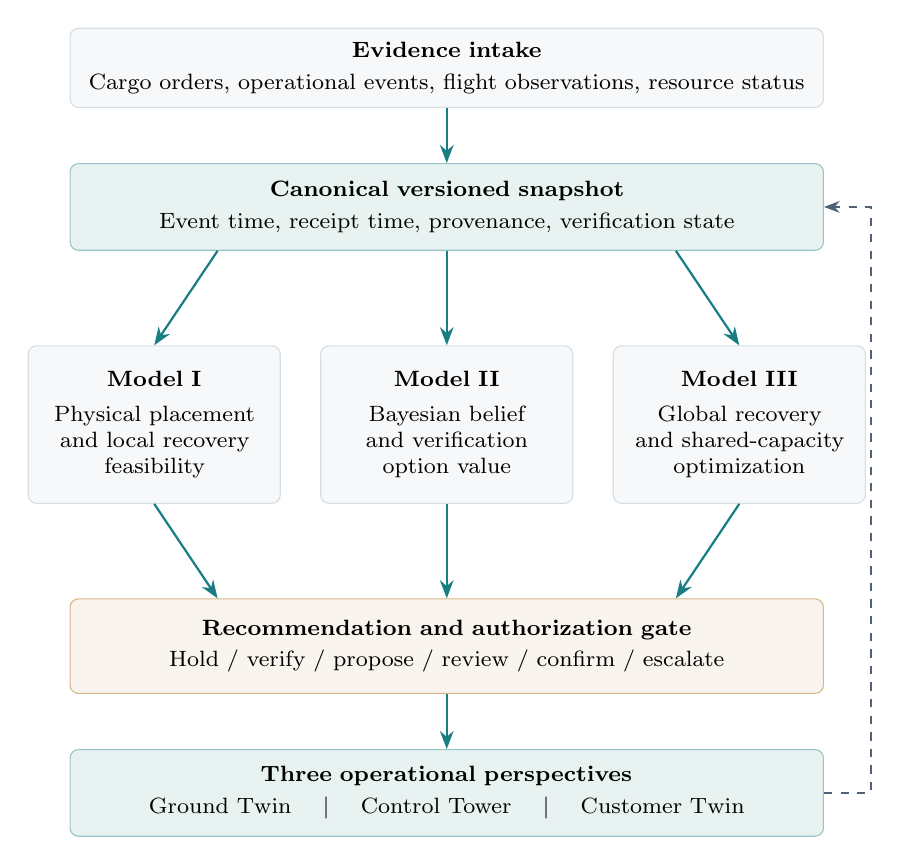
\begin{tikzpicture}[
  node distance=6mm,
  every node/.style={font=\footnotesize},
  >=Stealth
]

% ------------------------------------------------------------
% 1. Evidence intake
% ------------------------------------------------------------

\node[
  process,
  text width=.76\linewidth,
  minimum height=10mm
] (source) {
  \textbf{Evidence intake}\\[2pt]
  Cargo orders, operational events,
  flight observations, resource status
};

% ------------------------------------------------------------
% 2. Canonical operational snapshot
% ------------------------------------------------------------

\node[
  evidence,
  text width=.76\linewidth,
  minimum height=11mm,
  below=7mm of source
] (snapshot) {
  \textbf{Canonical versioned snapshot}\\[2pt]
  Event time, receipt time, provenance,
  verification state
};

% ------------------------------------------------------------
% 3. Three mathematical models
% ------------------------------------------------------------

\node[
  process,
  text width=.235\linewidth,
  minimum height=20mm,
  below=12mm of snapshot
] (m2) {
  \textbf{Model II}\\[3pt]
  Bayesian belief\\
  and verification\\
  option value
};

\node[
  process,
  text width=.235\linewidth,
  minimum height=20mm,
  left=5mm of m2
] (m1) {
  \textbf{Model I}\\[3pt]
  Physical placement\\
  and local recovery\\
  feasibility
};

\node[
  process,
  text width=.235\linewidth,
  minimum height=20mm,
  right=5mm of m2
] (m3) {
  \textbf{Model III}\\[3pt]
  Global recovery\\
  and shared-capacity\\
  optimization
};

% ------------------------------------------------------------
% 4. Recommendation and authorization
% ------------------------------------------------------------

\node[
  restricted,
  text width=.76\linewidth,
  minimum height=12mm,
  below=12mm of m2
] (gate) {
  \textbf{Recommendation and authorization gate}\\[2pt]
  Hold / verify / propose / review /
  confirm / escalate
};

% ------------------------------------------------------------
% 5. Three digital-twin perspectives
% ------------------------------------------------------------

\node[
  evidence,
  text width=.76\linewidth,
  minimum height=11mm,
  below=7mm of gate
] (twins) {
  \textbf{Three operational perspectives}\\[2pt]
  Ground Twin
  \quad $|$ \quad
  Control Tower
  \quad $|$ \quad
  Customer Twin
};

% ------------------------------------------------------------
% 6. Evidence flow
% ------------------------------------------------------------

\draw[flowarrow]
  (source.south) -- (snapshot.north);

% Snapshot -> Model I / II / III
\draw[flowarrow]
  ([xshift=-.24\linewidth]snapshot.south)
  -- (m1.north);

\draw[flowarrow]
  (snapshot.south)
  -- (m2.north);

\draw[flowarrow]
  ([xshift=.24\linewidth]snapshot.south)
  -- (m3.north);

% Models -> Recommendation gate
\draw[flowarrow]
  (m1.south)
  -- ([xshift=-.24\linewidth]gate.north);

\draw[flowarrow]
  (m2.south)
  -- (gate.north);

\draw[flowarrow]
  (m3.south)
  -- ([xshift=.24\linewidth]gate.north);

% Authorization -> Twin projections
\draw[flowarrow]
  (gate.south) -- (twins.north);

% ------------------------------------------------------------
% 7. Feedback loop (kept inside page margins)
% ------------------------------------------------------------

\draw[
  -{Stealth[length=2mm]},
  dashed,
  semithick,
  draw=Slate
]
  (twins.east)
  -- ++(6mm,0)
  |- (snapshot.east);

\end{tikzpicture}

\caption{
Integrated information-to-action architecture.
Versioned evidence informs three complementary
mathematical models; certified recommendations
are projected into synchronized digital twins.
Operational feedback generates new evidence,
while physical execution remains subject to
independent authorization and validation.
}
\label{fig:architecture}

\end{figure}

\researchnote{Interpretation.}{
The arrows in Figure~\ref{fig:architecture}
express required information dependencies.
They do not imply that the prototype already
re-solves every stochastic branch or performs
certified physical actuation.
}

% ============================================================
\section{Model I: Recovery-Aware Cargo Arrangement}
% ============================================================

\subsection{Physical decision space}

Let \(I\) denote cargo pieces and \(U\) eligible
unit-load devices.
Piece \(i\) is represented by a compact body

\[
K_i\subset\RR^3,
\qquad
m_i>0,
\qquad
c_i\in\RR^3.
\]

ULD \(u\) has an admissible loading region
\(G_u\subset\RR^3\).

A geometrically admissible placement satisfies

\begin{equation}
R_iK_i+p_i\subseteq G_u,
\qquad
R_i\in SO(3),
\label{eq:placement}
\end{equation}

where

\[
SO(3)=
\{R:R^\top R=I,\ \det R=1\}.
\]

A true executable assignment additionally requires
non-overlap, mass limits, stability,
approved restraints, compatible cargo,
physical handling paths and
operator-specific aircraft constraints.

For computational purposes,
Model I constructs a finite library
of physically admissible candidates
\(\mathcal A_i\).

The theoretical model assumes these candidates
have been properly certified.
A purely geometric bounding-box check
does not supply that certification.

\subsection{Two-stage uncertainty and recourse}

Let \(z\) be the initial plan and
\(\omega\in\Omega\) a disruption scenario.

Let

\[
\mathcal R_\omega(z)
\]

denote the legal, physically feasible repair
decisions remaining after scenario \(\omega\),
including frozen irreversible work.

The optimal recovery loss is

\begin{equation}
L(z,\omega)=
\min_{y\in\mathcal R_\omega(z)}
\left\{
\sum_{i\in I}
w_i\bigl(1-r_i(y,\omega)\bigr)
+\kappa d(z,y)
\right\}.
\label{eq:recourse}
\end{equation}

Here \(r_i\) is a service-success indicator,
\(w_i>0\) is an approved service weight,
and \(d(z,y)\) measures rehandling
and schedule changes.

The initial decision is shared across scenarios.
Allowing each scenario to choose a separate
initial arrangement would introduce
anticipative information.

\subsection{Buying flexibility at a bounded price}

Let \(N(z)\) be nominal missed-service loss
and \(C(z)\) ordinary nominal operating cost.

Define the lexicographic nominal optimum

\begin{align}
N^*
&=
\min_{z\in\mathcal Z_{\mathrm{safe}}}N(z),
\\
C^*
&=
\min_{\substack{
z\in\mathcal Z_{\mathrm{safe}}\\
N(z)=N^*
}}
C(z).
\end{align}

For an allowed additional nominal cost
\(\Delta\geq0\), define

\begin{equation}
\mathcal Z_\Delta=
\left\{
z\in\mathcal Z_{\mathrm{safe}}:
N(z)=N^*,
\ C(z)\leq C^*+\Delta
\right\}.
\label{eq:nominalbudget}
\end{equation}

The central objective is

\begin{equation}
\min_{z\in\mathcal Z_\Delta}
\left[
\CVaR_\alpha(L(z,\cdot))
+
\lambda\EE L(z,\cdot)
\right],
\label{eq:model1}
\end{equation}

with \(\lambda>0\).

For an integrable loss \(X\),

\begin{equation}
\CVaR_\alpha(X)
=
\min_{\eta\in\RR}
\left\{
\eta+
\frac{\EE(X-\eta)_+}{1-\alpha}
\right\}.
\label{eq:cvar}
\end{equation}

\subsection{Mathematical improvement guarantees}

\begin{theorem}[
Budgeted weak dominance
\cite{relaymodel1}
]
Let \(z_0\) be a nominal lexicographic
optimizer and let \(z_\Delta\)
minimize \eqref{eq:model1} over a finite,
nonempty \(\mathcal Z_\Delta\).
Then

\[
\rho_\alpha(L(z_\Delta,\cdot))
\leq
\rho_\alpha(L(z_0,\cdot)),
\]

where

\[
\rho_\alpha(X)=
\CVaR_\alpha(X)+\lambda\EE X.
\]
\end{theorem}

\begin{proof}
Because \(z_0\in\mathcal Z_\Delta\),
the optimal objective over
\(\mathcal Z_\Delta\) cannot exceed
the objective at \(z_0\).
\end{proof}

This theorem guarantees
\emph{non-worsening of the specified
risk objective within the same feasible set}.
It does not guarantee universal strict
improvement or real-world savings.

\begin{theorem}[
Sufficient strict-improvement criterion
\cite{relaymodel1}
]
For an alternative \(z_1\in\mathcal Z_\Delta\),
let

\[
D=L(z_1,\cdot)-L(z_0,\cdot),
\]

\[
G=\EE(-D)_+,
\qquad
H=\EE(D)_+.
\]

If

\begin{equation}
\lambda G>
\left(
\lambda+\frac{1}{1-\alpha}
\right)H,
\label{eq:strict}
\end{equation}

then the risk-aware optimum strictly improves
the objective of \(z_0\).
\end{theorem}

\begin{proof}
By monotonicity and subadditivity,

\[
\CVaR_\alpha(L(z_1))
-
\CVaR_\alpha(L(z_0))
\leq
\frac{H}{1-\alpha}.
\]

Also,

\[
\EE[L(z_1)-L(z_0)]=H-G.
\]

Therefore,

\[
\rho_\alpha(L(z_1))
-
\rho_\alpha(L(z_0))
\leq
\left(
\lambda+\frac{1}{1-\alpha}
\right)H-\lambda G.
\]

Condition \eqref{eq:strict}
makes the right-hand side negative.
Optimality of \(z_\Delta\) completes the result.
\end{proof}

\subsection{A physical worked example}

The original Model I paper considers
three unit-box pieces in a front-access lane.

Two admissible arrangements are

\[
z_A=A|B|C,
\qquad
z_B=C|B|A.
\]

The door is on the left.
Removing a targeted piece requires
temporarily moving pieces in front of it.

The scenario data are

\begin{table}[!htbp]
\centering
\caption{
Original Model I three-piece synthetic example.
}
\small
\begin{tabular}{@{}lrrr@{}}
\toprule
Scenario & Probability &
\(L(z_A,\omega)\) &
\(L(z_B,\omega)\) \\
\midrule
No inspection & 0.80 & 0 & 0 \\
Inspect C & 0.15 & 2 & 0 \\
Inspect A & 0.05 & 0 & 2 \\
\bottomrule
\end{tabular}
\end{table}

The expected losses are

\[
\EE L(z_A)=0.30,
\qquad
\EE L(z_B)=0.10.
\]

At \(\alpha=0.90\),

\[
\CVaR_{0.90}(L(z_A))=2,
\qquad
\CVaR_{0.90}(L(z_B))=1.
\]

With \(\lambda=1\),

\[
\rho_{0.90}(z_A)=2.30,
\qquad
\rho_{0.90}(z_B)=1.10.
\]

The second arrangement incurs one extra
nominal preparation unit
but reduces expected recovery loss by

\[
\frac{0.30-0.10}{0.30}
=
\boxed{66.7\%}
\]

and the CVaR component by \(50\%\).

\begin{figure}[!htbp]
\centering

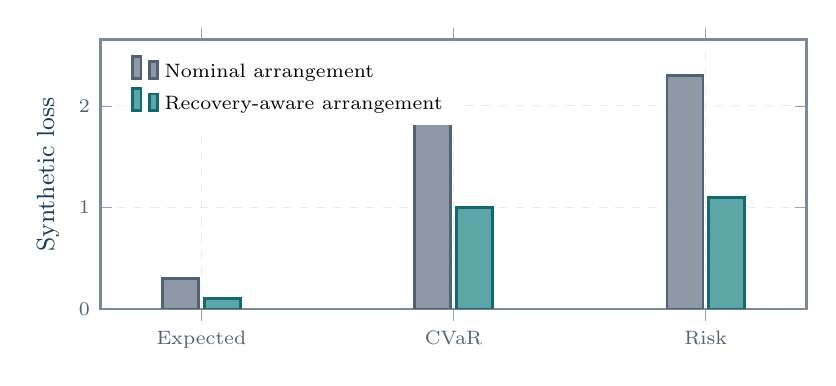
\begin{tikzpicture}
\begin{axis}[
  relayaxis,
  width=.87\linewidth,
  height=5.0cm,
  ybar,
  bar width=13pt,
  ymin=0,
  ymax=2.65,
  ylabel={Synthetic loss},
  symbolic x coords={Expected,CVaR,Risk},
  xtick=data,
  enlarge x limits=.20,
  legend pos=north west
]
\addplot[
  fill=Slate!65,
  draw=Slate
]
coordinates {
  (Expected,0.30)
  (CVaR,2.00)
  (Risk,2.30)
};

\addplot[
  fill=Teal!70,
  draw=DarkTeal
]
coordinates {
  (Expected,0.10)
  (CVaR,1.00)
  (Risk,1.10)
};

\legend{
  Nominal arrangement,
  Recovery-aware arrangement
}
\end{axis}
\end{tikzpicture}

\caption{
Computed Model I example.
The comparison is exact for this
three-piece synthetic physical instance.
}
\label{fig:model1-example}
\end{figure}

\researchnote{Scope limitation.}{
The executable RELAY prototype
implements bounded 2D candidate-library
optimization and a separate 3D box preflight.
It does not implement the full
certified three-dimensional stochastic
recourse model of this section.
}

% ============================================================
\section{Model II: PIVOT and the Value of Verification}
% ============================================================

\subsection{Why information can destroy optionality}

An apparently useful inspection can
consume the remaining time before
a recovery flight closes.

Accordingly, the value of verification
must include both information gained
and alternatives lost.

Let \(X\) be the hidden operational state,
\(b\) its prior distribution,
\(D_0\) the current decision set
and \(Z\) a proposed inspection observation.

After observing \(Z=z\),
the surviving decision set is \(D_z\).

\subsection{Bayesian decision risk}

Define the immediate Bayes risk

\begin{equation}
R_0=
\min_{d\in D_0}
\EE_b[\ell_0(d,X)].
\label{eq:immediate-risk}
\end{equation}

If an inspection \(q\) costs \(c_q\),
its optimal expected cost is

\begin{equation}
J_q=
c_q+
\sum_z
\PP(Z=z)
\min_{d\in D_z}
\EE[\ell_q(d,X,z)\mid Z=z].
\label{eq:verification-risk}
\end{equation}

The original research derives an exact
decomposition rather than a heuristic
information score.

\begin{theorem}[
PIVOT verification-value identity
\cite{relaymodel2}
]
For finite state, observation and decision
spaces with the loss functions defined
above,

\begin{equation}
R_0-J_q
=
I_q-A_q-B_q-c_q.
\label{eq:pivot-identity}
\end{equation}

Here:

\begin{itemize}[leftmargin=18pt,itemsep=2pt]
\item \(I_q\) is avoidable regret
from acting before observing \(Z\);
\item \(A_q\) is the effect of
changed post-inspection option sets;
\item \(B_q\) is the effect of
delay and changed downstream losses;
\item \(c_q\) is direct verification cost.
\end{itemize}

In particular, verification is strictly preferable
to the immediate optimum exactly when

\[
I_q>A_q+B_q+c_q.
\]
\end{theorem}

\begin{proof}[Proof principle]
Condition on each possible observation.
Starting from the immediate optimal action,
add and subtract the best decision in
the original option set and the best
decision in the post-inspection option set.
The tower property of conditional expectation
produces \eqref{eq:pivot-identity}.
No independence assumption is needed
for the general identity.
\end{proof}

An important subtlety is that
\(A_q\) and \(B_q\) need not be positive:
verification may reveal new alternatives
or coincide with improving external conditions.

\subsection{Bayesian updating}

Let \(H_1\) denote a material discrepancy
and \(H_0\) the aligned state.

For an inspection signal \(Y\),

\begin{equation}
\PP(H_1\mid Y=y)
=
\frac{
  \PP(Y=y\mid H_1)\PP(H_1)
}{
  \sum_{h\in\{H_0,H_1\}}
  \PP(Y=y\mid h)\PP(h)
}.
\label{eq:bayes}
\end{equation}

Such probabilities can support a
service decision.
They cannot independently authorize
an aircraft loading or a dangerous-goods action.

\subsection{A computed expiry threshold}

The original PIVOT example assumes

\[
\PP(H_1)=0.30
\]

and the illustrative loss matrix

\[
\begin{array}{c|cc}
& H_0 & H_1\\
\hline
\text{Keep/safe fallback} & 0 & 100\\
\text{Approved alternative} & 18 & 22
\end{array}.
\]

Without inspection,

\[
R(\text{keep})=30,
\qquad
R(\text{switch})=19.2.
\]

Inspection sensitivity is \(0.9\),
and its false-positive probability is \(0.2\).

The signal probabilities are

\[
\PP(Y=+)=0.41,
\qquad
\PP(Y=-)=0.59.
\]

Bayesian updating yields

\[
\PP(H_1\mid +)=0.65854,
\]

\[
\PP(H_1\mid -)=0.05085.
\]

The unconditional service cost
after an inspection, before inspection
expense and expiry, is

\[
R_Y=11.46.
\]

With inspection and delay cost \(3\)
and synthetic independent expiry probability
\(\rho\), the verification cost is

\begin{equation}
J_q(\rho)=14.46+18.54\rho.
\label{eq:expiry}
\end{equation}

Verification is preferable if

\begin{equation}
\rho<
\frac{19.20-14.46}{18.54}
=
\boxed{0.25566}.
\end{equation}

\begin{figure}[!htbp]
\centering

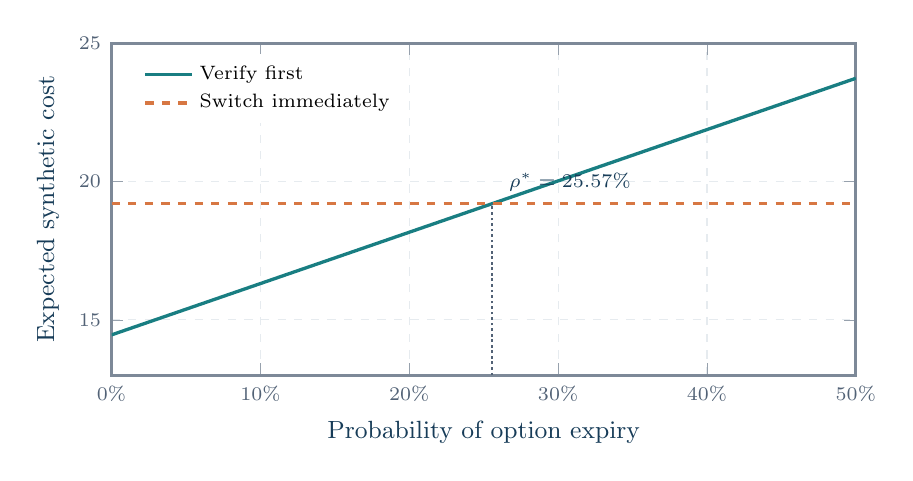
\begin{tikzpicture}
\begin{axis}[
  relayaxis,
  width=.91\linewidth,
  height=5.8cm,
  xmin=0,
  xmax=.50,
  ymin=13,
  ymax=25,
  xlabel={Probability of option expiry},
  ylabel={Expected synthetic cost},
  xtick={0,.1,.2,.3,.4,.5},
  xticklabels={0\%,10\%,20\%,30\%,40\%,50\%},
  legend pos=north west
]

\addplot[
  color=Teal,
  very thick,
  domain=0:.5,
  samples=70
]
{14.46+18.54*x};

\addplot[
  color=Orange,
  very thick,
  dashed,
  domain=0:.5
]
{19.2};

\addplot[
  color=Slate,
  densely dotted
]
coordinates {
  (.25566,13)
  (.25566,19.2)
};

\node[
  font=\scriptsize,
  anchor=south west,
  color=Navy
]
at (axis cs:.260,19.25)
{\(\rho^*=25.57\%\)};

\legend{
  Verify first,
  Switch immediately
}

\end{axis}
\end{tikzpicture}

\caption{
PIVOT decision reversal.
More information is not automatically
more valuable when recovery options expire.
All values are illustrative.
}
\label{fig:pivot-expiry}
\end{figure}

\subsection{The intended sequential controller}

For a fully dynamic system,
the belief-state is

\[
\xi_k=(b_k,Q_k,m_k,t_k),
\]

where \(Q_k\) records independently
authenticated context and \(m_k\)
records irreversible commitments.

The paper formulates a finite-horizon
semi-Markov recursion

\begin{equation}
V_k(\xi)=
\min_{a\in\mathcal A_{\mathrm{cert}}(\xi)}
\left\{
\EE[c(X,\xi,a)]
+
\EE\!\left[
V_{k+1}(\xi')
\mid \xi,a
\right]
\right\},
\label{eq:bellman}
\end{equation}

with a terminal expected-loss condition.

The admissible action set includes only
independently certified actions.

The implemented prototype evaluates a
finite one-step Bayesian controller;
it does not yet solve
\eqref{eq:bellman} over a calibrated
multi-stage operational transition model.

% ============================================================
\section{Model III: Global Recovery and Certified Exchanges}
% ============================================================

\subsection{Why independent recovery can fail}

Suppose two shipments each have
an inexpensive direct option,
but both options consume the last
unit of the same remaining flight capacity.

Independent shortest-path optimization
would select both, producing an
infeasible joint plan.

This is the central obstruction
addressed by Model III.

\subsection{Time-expanded recovery graph}

Let

\[
G_i=(V_i,E_i)
\]

be a time-expanded graph for shipment \(i\).

A vertex can represent

\[
(\text{station},\text{time},
\text{stage},\text{cargo condition}).
\]

Typed edges can represent inspection,
screening, build-up, flights,
transfers, trucking, customs and release.

Let \(\mathcal P_i(\theta)\)
contain paths satisfying the
currently known mandatory guards.

A path is executable only when its
physical, regulatory,
operational and booking conditions
have been independently confirmed.

\subsection{Finite-column global master}

Let \(y_{ip}\in\{0,1\}\)
indicate selection of route \(p\)
for shipment \(i\).

The restricted global assignment problem is

\begin{equation}
\begin{aligned}
\min_y\quad
& \sum_i\sum_{p\in\mathcal P_i}c_{ip}y_{ip}\\
\text{s.t.}\quad
& \sum_{p\in\mathcal P_i}y_{ip}=1
&&\forall i,\\
& Ay\leq C,\\
& Dy\leq d,\\
& y_{ip}\in\{0,1\}.
\end{aligned}
\label{eq:global-milp}
\end{equation}

The model includes an explicitly
labelled unresolved or escalation
option when authorized.

Here \(A\) describes shared flight,
handling and cold-chain resource use;
\(C\) is available modeled capacity;
and \(Dy\leq d\) represents
additional valid coupling constraints.

\begin{proposition}[
Exactness within a complete
candidate representation
\cite{relaymodel3}
]
If the route candidates cover all
permitted itineraries for a fixed
snapshot, and every relevant joint
constraint is represented,
an optimum of
\eqref{eq:global-milp}
is an optimum among those
permitted joint itinerary selections.
\end{proposition}

The completeness assumption matters.
An optimal solver status over
53 enumerated candidates
does not prove optimality over
all physically possible routes.

\subsection{Integer-kernel exchange geometry}

After exact integer scaling and
bounded slack-variable introduction,
a finite recovery master can be written

\begin{equation}
\min
\left\{
w^\top v:
Mv=b,\ 
\ell\leq v\leq u,\ 
v\in\ZZ^m
\right\}.
\label{eq:integer-master}
\end{equation}

A feasible exchange direction \(g\)
preserves

\begin{equation}
Mg=0,
\qquad
\ell\leq v+g\leq u.
\label{eq:kernel}
\end{equation}

A Graver basis
\(\mathcal G(M)\)
contains the conformally minimal
nonzero integer-kernel directions.

The original research connects
these directions to genuine
cluster-algebra exchange relations.

For a rank-one seed associated with \(g\),

\begin{equation}
X_gX'_g
=
U^{g^+}+U^{g^-},
\label{eq:cluster}
\end{equation}

where

\[
g_j^+=\max(g_j,0),
\qquad
g_j^-=\max(-g_j,0).
\]

Under the frozen-coefficient specialization

\[
U_j=\exp(-\beta w_j),
\qquad
\beta>0,
\]

the monomial ratio satisfies

\begin{equation}
R_g
=
\frac{U^{g^+}}{U^{g^-}}
=
\exp(-\beta w^\top g).
\label{eq:mutation-gain}
\end{equation}

Consequently,

\[
R_g>1
\quad\Longleftrightarrow\quad
w^\top(v+g)<w^\top v.
\]

\subsection{The full-basis improvement theorem}

\begin{theorem}[
Certified Graver-encoded augmentation
\cite{relaymodel3}
]
Consider a nonempty, bounded integer-linear
feasible set of the form
\eqref{eq:integer-master}.

If a feasible \(v\) is not globally optimal,
then an improving feasible direction
\(g\in\mathcal G(M)\) exists.

Conversely, if no such improving direction exists,
\(v\) is globally optimal.

An algorithm repeatedly applying
strictly improving moves terminates
at a global optimum provided
the full relevant Graver basis is searched.
\end{theorem}

\begin{proof}[Proof sketch]
Choose a better feasible solution \(v^*\).
The difference \(h=v^*-v\)
belongs to the integer kernel.
A conformal Graver decomposition
writes

\[
h=g^1+\cdots+g^r.
\]

Every \(v+g^j\) remains
within the bounds, since the
directions are conformal to \(h\).

Furthermore,

\[
\sum_jw^\top g^j
=
w^\top(v^*-v)<0.
\]

At least one direction must be improving.
Finite termination follows from strict
cost decrease over the bounded integer set.
\end{proof}

The optimality guarantee relies on
standard Graver augmentation theory
and faithful cluster encoding.

It does not imply that constructing
or searching the full basis is cheap.

\subsection{A computed shared-slot example}

The original Model III research considers
two shipments and one remaining direct-flight slot.

\begin{table}[!htbp]
\centering
\caption{Original Model III synthetic example.}
\small
\begin{tabular}{@{}lrr@{}}
\toprule
Shipment & Direct cost & Fallback cost \\
\midrule
A & 1 & 4 \\
B & 1 & 8 \\
\bottomrule
\end{tabular}
\end{table}

Allocating the direct slot to A costs

\[
1+8=9.
\]

Allocating it to B costs

\[
4+1=5.
\]

The joint exchange

\[
g=(-1,1,1,-1,0)^\top
\]

has exact objective change

\[
w^\top g=-4.
\]

Thus the improved joint allocation reduces
this example's nominal cost by

\begin{equation}
\frac{9-5}{9}\times100\%
=
\boxed{44.4\%}.
\end{equation}

This demonstrates opportunity-cost-aware
capacity allocation.
It is a small constructed example,
not a measured airline recovery improvement.

\subsection{Correlated disruption risk}

A system-wide stochastic objective can take the form

\begin{equation}
\min_{y\in\mathcal Y_{\mathrm{safe}}}
\left[
\lambda\EE L_\omega(y)
+
\CVaR_\alpha(L_\omega(y))
+
\gamma\Delta_{\mathrm{global}}(y,y_0)
\right].
\label{eq:global-cvar}
\end{equation}

Correlated weather, congestion or
network shocks must be represented
using joint scenarios rather than
unjustified independence assumptions.

\researchnote{Implementation boundary.}{
The final software uses SciPy/HiGHS
on finite candidate itinerary columns
and evaluates synthetic risk scenarios.
Cluster/Graver exchange is represented
as a mathematical research fixture;
the operational runtime is
\emph{not} a complete Graver-basis
augmentation algorithm.
}

% ============================================================
\section{Integrating the Three Models}
% ============================================================

\subsection{One decision, three distinct questions}

Model I concerns physical feasibility
and recourse.
Model II concerns the value and timing
of information.
Model III concerns shared network allocation.

A correct controller must not simply
concatenate their independent outputs.

In particular, if Model II places
shipment \(i\) on HOLD,
any unconfirmed executable route for \(i\)
must be removed or conditioned,
and the remaining shared capacity
may need to be re-optimized.

\subsection{The ideal closed-loop formulation}

Let \(a_t\) be an operational action
and \(\mathcal A_{\mathrm{cert}}(\theta_t)\)
the externally certified action set.

A conceptual integrated policy is

\begin{equation}
\pi^*(\theta_t)
\in
\argmin_{a_t\in
\mathcal A_{\mathrm{cert}}(\theta_t)}
\left\{
\text{immediate cost}
+
\text{risk-adjusted future loss}
\right\},
\label{eq:integrated-policy}
\end{equation}

subject to physical, informational,
capacity, irreversibility
and authorization constraints.

This expression defines a
\emph{research target}.
The final prototype
does not solve it exactly.

\subsection{Operational algorithm}

\begin{enumerate}[
  label=\textbf{Step \arabic*.},
  leftmargin=22pt,
  itemsep=3pt
]

\item
Ingest an event and preserve its
source, version, event time and receipt time.

\item
Reconstruct a causally valid,
immutable as-of snapshot.

\item
Separate observed,
tentative, verified,
confirmed and unknown facts.

\item
Generate physical placement and
local-recovery candidates from Model I.

\item
Generate candidate network paths
and solve the shared-capacity master
using Model III.

\item
Use Model II to evaluate
verification, holding and
available recovery decisions.

\item
Reconcile HOLD/VERIFY gates with
capacity allocation and, where necessary,
re-solve the global master.

\item
Reject unsafe, stale,
unauthorized or unconfirmed
physical proposals.

\item
Send a recommendation through the
appropriate approval and confirmation workflow.

\item
Append the resulting evidence and update
Ground, Control Tower and Customer projections.

\end{enumerate}

\subsection{Important safety invariants}

A deployable implementation should maintain

\begin{align}
\text{Physical execution}
&\Longrightarrow
\text{current certification},
\\
\text{Booked capacity}
&\Longrightarrow
\text{carrier confirmation},
\\
\text{Approved action}
&\Longrightarrow
\text{authorized approver},
\\
\text{Customer confirmed status}
&\Longrightarrow
\text{confirmed source evidence}.
\end{align}

A recommendation is not an execution.
An internal simulation approval is not
an airline booking confirmation.

These distinctions are part of
the product's mathematical
and engineering correctness.

% ============================================================
\section{From Research to an Executable Product}
% ============================================================

\subsection{Development trajectory}

The project evolved through twelve main versions
and one operational hotfix.

\begin{figure}[!htbp]
\centering

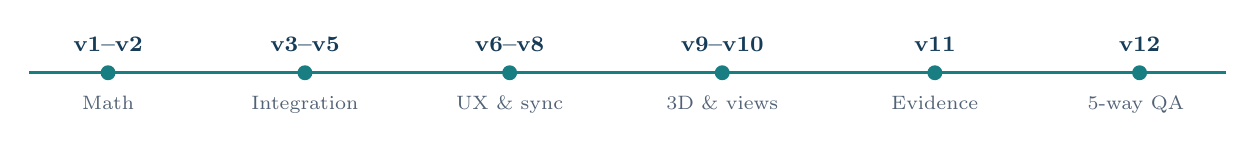
\begin{tikzpicture}[
  x=1cm,
  y=1cm
]

\draw[
  very thick,
  color=Teal
]
(0,0)--(15.2,0);

\foreach \x/\label/\phase in {
  1/{v1--v2}/{Math},
  3.5/{v3--v5}/{Integration},
  6.1/{v6--v8}/{UX \& sync},
  8.8/{v9--v10}/{3D \& views},
  11.5/{v11}/{Evidence},
  14.1/{v12}/{5-way QA}
}{
  \fill[Teal] (\x,0) circle(2.7pt);
  \node[
    anchor=south,
    font=\footnotesize\bfseries,
    text=Navy
  ] at (\x,.15){\label};
  \node[
    anchor=north,
    font=\scriptsize,
    text=Slate,
    align=center
  ] at (\x,-.17){\phase};
}

\end{tikzpicture}

\caption{
Research-to-product development milestones.
Version progression records increasing
software and experimental scope,
not airline certification.
}
\label{fig:journey}
\end{figure}

\begin{table}[!htbp]
\centering
\caption{Engineering development from v1 to v12.}
\label{tab:versions}
\small
\begin{tabularx}{\linewidth}{@{}p{16mm}L@{}}
\toprule
\textbf{Version} & \textbf{Principal contribution} \\
\midrule
v1--v2 &
Three mathematical backend modules,
event data, FastAPI,
initial safety and review gates. \\
v3--v3.1 &
First integrated full-stack digital twin;
fixed live dispatch failure behavior. \\
v4 &
Canonical shipment identities,
shared synthetic evidence and clock. \\
v5 &
Provenance audits,
OAG-compatible synthetic adapter,
explicit mathematical validity boundaries. \\
v6 &
Light-theme, three-perspective
Ground/Control/Customer product interface. \\
v7 &
Richer staging scenarios,
3D bounding-box preflight,
effectiveness experiments. \\
v8 &
Shared server-side simulation controller,
automatic synchronized updates. \\
v9 &
WebGL2 ground geometry,
camera control, weather and animations. \\
v10 &
Dynamic scene presentation,
mathematical visual cards,
multi-route customer globe. \\
v11 &
Full-cohort staging benchmark,
percentage KPIs, statistical convergence,
tail risk and hypothetical ROI. \\
v12 &
Five synchronized selectable policy worlds,
two hybrid policies,
final common-input holdout and QA. \\
\bottomrule
\end{tabularx}
\end{table}

\subsection{The three product perspectives}

The final application retains three
operationally meaningful views.

\subsubsection{Ground Twin}

A visual simulation of cargo arrival,
staging queues, handling resources,
equipment, aircraft stands and
synthetic disruptions.

Users can compare what happens under
different scheduling decisions
while sharing the same generated input stream.

\subsubsection{Control Tower}

A decision-support interface presenting
current incidents, proposed actions,
approval states and Before/After impact.

The interface provides progressive access
to mathematical explanations,
scenario costs, model status,
process logs and candidate routes.

\subsubsection{Customer Twin}

A shipment-oriented projection
of observed milestones,
route candidates, estimated arrival
and recovery communications.

Its state language separates:

\begin{center}
\small
Observed
\quad $\rightarrow$ \quad
Under review
\quad $\rightarrow$ \quad
Proposed
\quad $\rightarrow$ \quad
Confirmed
\quad $\rightarrow$ \quad
Executed.
\end{center}

Only independently confirmed changes
should be presented as confirmed
in a real deployment.

\subsection{Five policy worlds}

Version 12 adds a separate
five-policy staging comparison:

\[
\Pi=
\{
\text{FCFS},
\text{v10},
\text{v11},
\text{Model A},
\text{EDF}
\}.
\]

The interface displays any
two, three, four or five policies
at a time.

All five policies still advance internally
on the same arrival stream and
simulation clock.

\researchnote{Critical distinction.}{
The five v12 Digital Twins compare
\emph{ground staging policies}.
They are not five simultaneous,
fully integrated executions of
the original three-paper
airline-wide stochastic optimizer.
The mathematical engine and original
three-perspective product remain
separate but related parts
of the research prototype.
}

% ============================================================
\section{Evidence Architecture and Synthetic Data}
% ============================================================

\subsection{Source data}

The 30-day historical synthetic catalog contains

\begin{table}[!htbp]
\centering
\caption{Synthetic historical input inventory.}
\label{tab:data-volume}
\small
\begin{tabular}{@{}lr@{}}
\toprule
Entity & Records \\
\midrule
Flights & 429 \\
Shipments & 636 \\
Physical pieces & 793 \\
ULD records & 14 \\
Historical events & 5,120 \\
\bottomrule
\end{tabular}
\end{table}

These are generated research records,
not measurements from a Cathay
production data feed.

\subsection{Event composition}

\begin{table}[!htbp]
\centering
\caption{Composition of the synthetic event ledger.}
\small
\begin{tabular}{@{}lr@{}}
\toprule
Event category & Count \\
\midrule
Shipment milestones & 3,409 \\
Flight state updates & 1,524 \\
Booking changes & 76 \\
Flight delays & 59 \\
Dimension conflicts & 38 \\
Flight cancellations & 8 \\
Terminal congestion & 6 \\
\midrule
\textbf{Total} & \textbf{5,120} \\
\bottomrule
\end{tabular}
\end{table}

\subsection{Causal evidence representation}

Each event should retain, where available,

\[
e=
(
\text{id},
\text{entity},
\text{source},
t_{\mathrm{event}},
t_{\mathrm{receipt}},
\text{revision},
\text{payload},
\text{status}
).
\]

Two times are essential:

\begin{itemize}[leftmargin=18pt,itemsep=2pt]
\item
\(t_{\mathrm{event}}\):
when the event purportedly occurred;
\item
\(t_{\mathrm{receipt}}\):
when RELAY received the observation.
\end{itemize}

A decision made at time \(t\)
must not use evidence received after \(t\).

A replayed snapshot is therefore based on
the information actually available
at the decision boundary.

\subsection{Synthetic data integrity findings}

The structural audit reported:

\begin{itemize}[leftmargin=18pt,itemsep=2pt]
\item zero duplicate primary IDs;
\item zero invalid piece-to-shipment references;
\item zero shipment/piece weight mismatches;
\item zero missing assigned-flight references;
\item zero event-time-after-receipt-time anomalies;
\item zero reported violations of
the checked event receipt ordering.
\end{itemize}

These checks support internal consistency.
They do not validate the statistical
representativeness of real operations.

\subsection{OAG and IATA integration boundaries}

OAG flight information can contribute
schedule, flight-status, airport,
equipment and connection evidence
\cite{oagportal}.

IATA ONE Record provides a
standardized cargo data model,
API framework and security concepts
\cite{onerecord}.

However,

\begin{equation}
\text{Published flight availability}
\not\Rightarrow
\text{Confirmed bookable cargo capacity}.
\end{equation}

Likewise,

\begin{equation}
\text{Electronic tracking event}
\not\Rightarrow
\text{Certified physical truth}.
\end{equation}

The implemented OAG bridge is a
clearly identified synthetic schema
illustration, not a live
licensed data connection.

A production adapter must obtain
authorized credentials, respect
data licensing, validate flight identity,
and independently confirm the
operational capacity and permission state.

% ============================================================
\section{Five Ground-Scheduling Policies}
% ============================================================

\subsection{Decision problem}

At each ground-handling decision epoch,
let \(\mathcal W_t\) be the waiting jobs
and \(B_r(t)\) the capacity
of resource \(r\).

A staging action \(x_t\)
must satisfy

\begin{equation}
\sum_{j\in\mathcal W_t}
a_{jr}x_{jt}
\leq B_r(t),
\qquad
x_{jt}\in\{0,1\}.
\label{eq:staging-resource}
\end{equation}

The simulation also applies
job eligibility and nonpreemptive
active-task accounting.

Different policies rank eligible
jobs differently;
they do not change the shared
generated workload.

\subsection{The five alternatives}

\begin{table}[!htbp]
\centering
\caption{Policies evaluated in the final experiment.}
\label{tab:policies}
\small
\begin{tabularx}{\linewidth}{@{}p{30mm}L@{}}
\toprule
Policy & Operational selection rule \\
\midrule
FCFS &
Oldest eligible task first;
reference baseline. \\
RELAY v10 &
Original observable urgency-based
selection heuristic. \\
RELAY v11 &
Deadline, priority and duration-aware
two-class staging triage;
conservative single-server fallback. \\
RELAY + Model A &
Experimental \emph{DeadlineGuard-A}
with stronger critical-priority
and deadline protection. \\
RELAY + EDF &
Experimental earliest-deadline-emphasis,
cost-first staging alternative. \\
\bottomrule
\end{tabularx}
\end{table}

Model A is an engineered
ground-scheduling policy,
not an external foundation model
and not the original mathematical Model I.

EDF is also a staging heuristic,
not a certified
three-model stochastic optimum.

\subsection{Why multiple policies matter}

No single operating rule is
guaranteed to dominate on every metric.

A lower modeled cost can coexist with
worse on-time performance;
a deadline-oriented policy may prioritize
service while slowing the clearance
of an existing backlog.

The five-way comparison is therefore
a practical multiobjective experiment:

\[
\min
\left(
\EE C,\ 
\CVaR_{0.9}(C),\
-\text{on-time rate},\
\text{lead time}
\right),
\]

where the displayed vector
represents competing evaluation criteria,
not a claim that the runtime solves
a fully specified multiobjective program.

% ============================================================
\section{Experimental Protocol}
% ============================================================

\subsection{Common-random-number design}

The final version-12 holdout uses

\[
6\text{ scenarios}
\times
500\text{ episodes}
=
3{,}000
\]

independently generated
common-input workload episodes.

Each workload is evaluated under
five policies, yielding

\[
3{,}000\times5
=
\boxed{15{,}000}
\]

policy outcome records.

The holdout seed is

\[
s=9099.
\]

All policies in a paired episode share
the same arrivals, task attributes
and exogenous disruption conditions.

This removes much of the noise
that would arise from comparing
unrelated random workloads.

\subsection{Time horizon and censored work}

The benchmark admits new work for
24 simulation ticks.

Each tick represents ten
synthetic operational minutes.

After admission stops,
the system permits up to 110 further
ticks to clear work.

Jobs still unfinished at the horizon
remain in the full-cohort
service denominator
and receive modeled outstanding-work costs.

This addresses an important weakness
of earlier 21-tick comparisons:
ignoring incomplete work can
artificially improve measured performance.

\subsection{Synthetic cost ledger}

For policy \(\pi\) and episode \(e\),
write the recorded modeled cost as

\begin{equation}
C_e^\pi
=
C_{\mathrm{handling}}
+
C_{\mathrm{waiting}}
+
C_{\mathrm{overdue}}
+
C_{\mathrm{lateness}}
+
C_{\mathrm{unfinished}}.
\label{eq:ledger}
\end{equation}

All components are synthetic
penalty units.

They have not been calibrated
to actual airline operating costs.

\subsection{Performance metrics}

The principal percentage cost reduction is

\begin{equation}
S_\pi=
100
\left(
1-
\frac{
\overline C_\pi
}{
\overline C_{\mathrm{FCFS}}
}
\right),
\label{eq:savings}
\end{equation}

where the denominator is the
\emph{mean FCFS cost over the same episodes}.

This is the ratio of sample means,
not the mean of episode-level percentages.

Let \(n_e\) be all admitted jobs
and \(o_e^\pi\) jobs meeting
their modeled service deadline.

The full-cohort on-time rate is

\begin{equation}
Q_\pi=
100\,
\frac{\sum_e o_e^\pi}
{\sum_e n_e}.
\label{eq:ontime}
\end{equation}

Service improvement in percentage points is

\begin{equation}
\Delta Q_\pi=
Q_\pi-Q_{\mathrm{FCFS}}.
\label{eq:pp}
\end{equation}

The adverse-episode probability is estimated by

\begin{equation}
\widehat p_{\mathrm{worse}}^\pi
=
\frac1N
\sum_{e=1}^{N}
\Ind\{
C_e^\pi>C_e^{\mathrm{FCFS}}
\}.
\label{eq:regression}
\end{equation}

For empirical tail risk,
the benchmark measures

\[
\widehat{\CVaR}_{0.90}
\]

over episode-total costs.

This is not the same random variable
as the internal Model III
network-scenario CVaR.

\subsection{Confidence intervals}

Paired bootstrap resampling
preserves the correspondence
between policies within an episode.

For each bootstrap sample \(b\),

\[
S_\pi^{(b)}
=
100
\left(
1-
\frac{
\overline C_\pi^{(b)}
}{
\overline C_{\mathrm{FCFS}}^{(b)}
}
\right).
\]

Empirical bootstrap quantiles
form the reported 95\%
sampling interval.

Such intervals measure finite-sample
uncertainty under the chosen generator.
They do not account for
model misspecification or
unknown real-airline distributions.

% ============================================================
\section{Final Results: Cost and Service Quality}
% ============================================================

\subsection{Normal operations}

The most informative
single-condition comparison is
the normal synthetic operating regime.

\begin{table}[!htbp]
\centering
\caption{
Final normal-operation five-policy
holdout, seed 9099, 500 episodes.
}
\label{tab:normal}
\small
\begin{adjustbox}{max width=\linewidth}
\begin{tabular}{@{}lrrrr@{}}
\toprule
Policy &
Mean cost &
Cost saved &
On-time rate &
CVaR$_{90}$ \\
&
(units) &
(\%) &
(\%) &
(units) \\
\midrule
FCFS &
1946.84 & 0.00 & 39.36 & 4279.24 \\
RELAY v10 &
1820.14 & 6.51 & 36.41 & 4164.85 \\
RELAY v11 &
1775.19 & 8.82 & 64.02 & 3757.37 \\
RELAY + Model A &
1723.60 & 11.47 & \textbf{64.04} & 3663.19 \\
RELAY + EDF &
\textbf{1605.65} &
\textbf{17.53} &
56.64 &
\textbf{3471.60} \\
\bottomrule
\end{tabular}
\end{adjustbox}
\end{table}

The best cost policy is EDF.

The highest on-time policy in this
experiment is Model A.

Relative to FCFS,
Model A improves on-time performance by

\[
64.04-39.36
=
\boxed{24.69\text{ percentage points}}.
\]

Yet EDF has a lower synthetic cost.
This is a genuine
cost--quality trade-off
under the specified modeled objective.

\subsection{Cost--quality frontier}

\begin{figure}[!htbp]
\centering

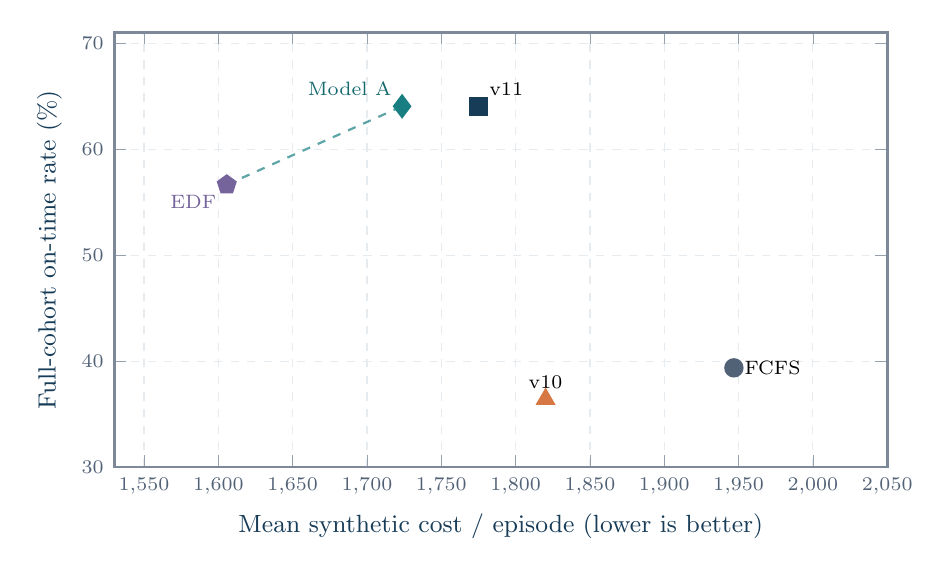
\begin{tikzpicture}
\begin{axis}[
  relayaxis,
  width=.94\linewidth,
  height=7.1cm,
  xmin=1530,
  xmax=2050,
  ymin=30,
  ymax=71,
  xlabel={Mean synthetic cost / episode
  (lower is better)},
  ylabel={Full-cohort on-time rate (\%)},
  legend pos=south west
]

\addplot[
  only marks,
  mark=*,
  mark size=3.0pt,
  color=Slate
]
coordinates {(1946.84,39.36)};

\addplot[
  only marks,
  mark=triangle*,
  mark size=3.2pt,
  color=Orange
]
coordinates {(1820.14,36.41)};

\addplot[
  only marks,
  mark=square*,
  mark size=3.0pt,
  color=Navy
]
coordinates {(1775.19,64.02)};

\addplot[
  only marks,
  mark=diamond*,
  mark size=3.7pt,
  color=Teal
]
coordinates {(1723.60,64.04)};

\addplot[
  only marks,
  mark=pentagon*,
  mark size=3.2pt,
  color=Purple
]
coordinates {(1605.65,56.64)};

\addplot[
  color=Teal!70,
  thick,
  dashed
]
coordinates {
  (1605.65,56.64)
  (1723.60,64.04)
};

\node[
  font=\scriptsize,
  anchor=west
]
at (axis cs:1946.84,39.36)
{FCFS};

\node[
  font=\scriptsize,
  anchor=south
]
at (axis cs:1820.14,36.41)
{v10};

\node[
  font=\scriptsize,
  anchor=south west
]
at (axis cs:1775.19,64.02)
{v11};

\node[
  font=\scriptsize,
  anchor=south east,
  color=DarkTeal
]
at (axis cs:1723.60,64.04)
{Model A};

\node[
  font=\scriptsize,
  anchor=north east,
  color=Purple
]
at (axis cs:1605.65,56.64)
{EDF};

\end{axis}
\end{tikzpicture}

\caption{
Synthetic cost--quality frontier.
The preferred region is upper-left.
EDF and Model A represent distinct
cost/service trade-offs;
the graph is not a monetary ROI frontier.
}
\label{fig:frontier}
\end{figure}

\subsection{Six operating conditions}

The final holdout includes
normal demand,
peak demand,
crew shortage,
cold-chain outage,
high resource capacity
and temporary disruption.

\begin{table}[!htbp]
\centering
\caption{
Cost reduction relative to FCFS,
all values in percent.
}
\label{tab:sixcost}
\small
\begin{adjustbox}{max width=\linewidth}
\begin{tabular}{@{}lrrrr@{}}
\toprule
Scenario &
v10 &
v11 &
Model A &
EDF \\
\midrule
Normal & 6.51 & 8.82 & 11.47 & \textbf{17.53} \\
Peak & 0.40 & 17.22 & 18.18 & \textbf{22.24} \\
Crew shortage & -0.37 & 0.00 & 0.00 & 0.00 \\
Cold outage & 1.15 & 2.50 & 2.79 & \textbf{3.74} \\
High capacity & 11.19 & 10.62 & 14.75 & \textbf{23.95} \\
Disruption & 1.93 & 10.07 & 10.88 & \textbf{15.88} \\
\bottomrule
\end{tabular}
\end{adjustbox}
\end{table}

\begin{figure}[!htbp]
\centering

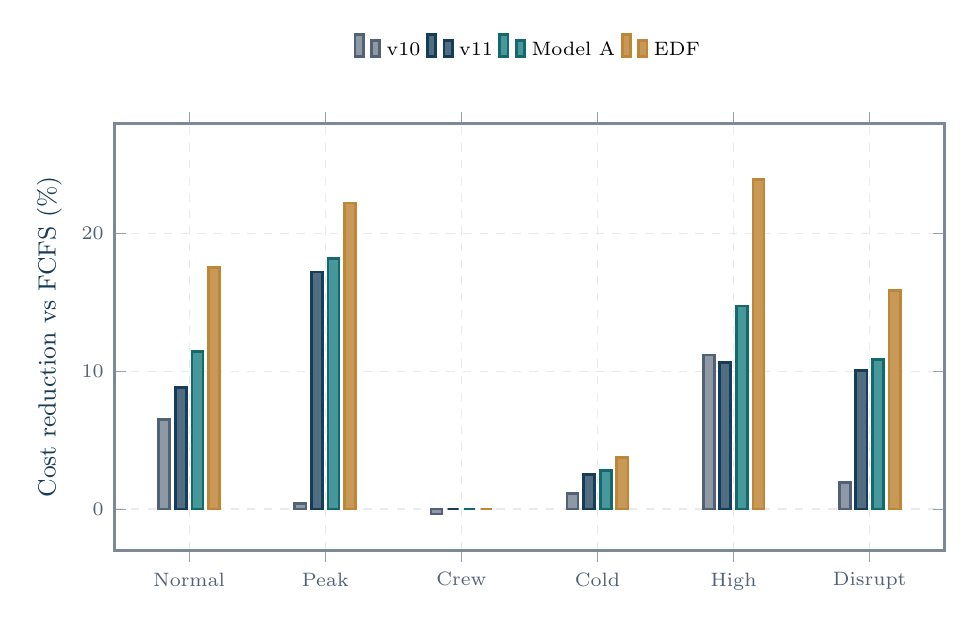
\begin{tikzpicture}
\begin{axis}[
  relayaxis,
  width=\linewidth,
  height=7.0cm,
  ybar,
  bar width=4pt,
  ymin=-3,
  ymax=28,
  ylabel={Cost reduction vs FCFS (\%)},
  symbolic x coords={
    Normal,
    Peak,
    Crew,
    Cold,
    High,
    Disrupt
  },
  xtick=data,
  enlarge x limits=.11,
  legend columns=4,
  legend style={
    at={(.5,1.12)},
    anchor=south,
    font=\scriptsize,
    draw=none
  }
]

\addplot[
  fill=Slate!65,
  draw=Slate
]
coordinates {
  (Normal,6.51)
  (Peak,.40)
  (Crew,-.37)
  (Cold,1.15)
  (High,11.19)
  (Disrupt,1.93)
};

\addplot[
  fill=Navy!75,
  draw=Navy
]
coordinates {
  (Normal,8.82)
  (Peak,17.22)
  (Crew,0)
  (Cold,2.50)
  (High,10.62)
  (Disrupt,10.07)
};

\addplot[
  fill=Teal!80,
  draw=DarkTeal
]
coordinates {
  (Normal,11.47)
  (Peak,18.18)
  (Crew,0)
  (Cold,2.79)
  (High,14.75)
  (Disrupt,10.88)
};

\addplot[
  fill=Gold!85,
  draw=Gold
]
coordinates {
  (Normal,17.53)
  (Peak,22.24)
  (Crew,0)
  (Cold,3.74)
  (High,23.95)
  (Disrupt,15.88)
};

\legend{
  v10,
  v11,
  Model A,
  EDF
}

\end{axis}
\end{tikzpicture}

\caption{
Five-way experiment:
percentage modeled cost improvement
relative to each scenario's FCFS baseline.
Negative values denote regressions.
}
\label{fig:six-cost}
\end{figure}

\subsection{Service quality under stress}

\begin{table}[!htbp]
\centering
\caption{
Full-cohort on-time performance
in the final holdout (\%).
}
\label{tab:service-all}
\small
\begin{adjustbox}{max width=\linewidth}
\begin{tabular}{@{}lrrrrr@{}}
\toprule
Scenario &
FCFS &
v10 &
v11 &
Model A &
EDF \\
\midrule
Normal &
39.36 & 36.41 & 64.02 & \textbf{64.04} & 56.64 \\
Peak &
11.99 & 8.96 & \textbf{39.79} & 39.31 & 28.84 \\
Crew shortage &
4.33 & 2.46 & 4.33 & 4.33 & 4.33 \\
Cold outage &
27.66 & 25.58 & \textbf{51.83} & 51.48 & 43.92 \\
High capacity &
48.05 & 46.27 & 76.88 & \textbf{77.20} & 73.80 \\
Disruption &
19.27 & 16.54 & 33.29 & \textbf{33.73} & 31.30 \\
\bottomrule
\end{tabular}
\end{adjustbox}
\end{table}

Under peak demand,
Model A reduces modeled cost by 18.18\%
but has a slightly lower on-time rate
than v11.

Therefore even the two closely related
RELAY policies should not be described
as a strict multiobjective dominance pair.

\subsection{Normalized normal-operation comparison}

\begin{figure}[!htbp]
\centering

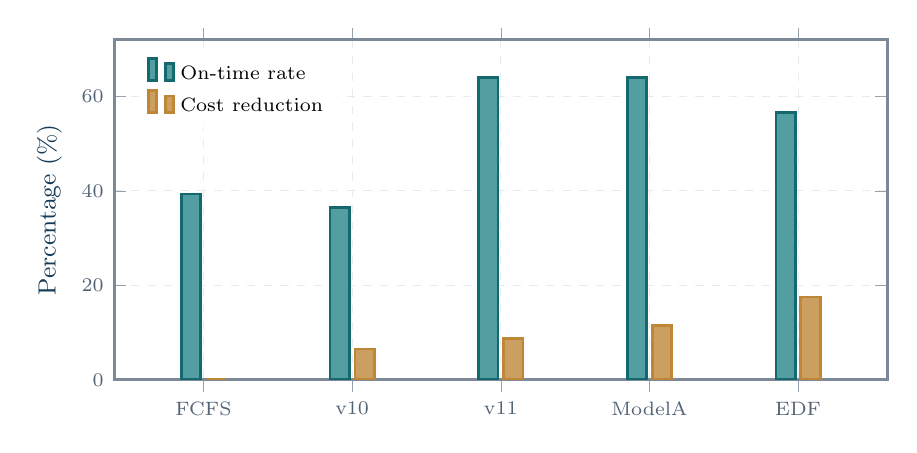
\begin{tikzpicture}
\begin{axis}[
  relayaxis,
  width=.94\linewidth,
  height=5.9cm,
  ybar,
  bar width=7pt,
  ymin=0,
  ymax=72,
  ylabel={Percentage (\%)},
  symbolic x coords={
    FCFS,
    v10,
    v11,
    ModelA,
    EDF
  },
  xtick=data,
  enlarge x limits=.15,
  legend pos=north west
]

\addplot[
  fill=Teal!75,
  draw=DarkTeal
]
coordinates {
  (FCFS,39.36)
  (v10,36.41)
  (v11,64.02)
  (ModelA,64.04)
  (EDF,56.64)
};

\addplot[
  fill=Gold!80,
  draw=Gold
]
coordinates {
  (FCFS,0)
  (v10,6.51)
  (v11,8.82)
  (ModelA,11.47)
  (EDF,17.53)
};

\legend{
  On-time rate,
  Cost reduction
}

\end{axis}
\end{tikzpicture}

\caption{
Normal synthetic operations:
service quality and modeled cost improvement
are different dimensions.
}
\label{fig:quality-cost-bars}
\end{figure}

% ============================================================
\section{Risk, Probability and Statistical Convergence}
% ============================================================

\subsection{Policy regressions}

A policy with lower average cost
can lose on individual episodes.

\begin{table}[!htbp]
\centering
\caption{
Fraction of normal-operation episodes
with higher cost than FCFS.
}
\small
\begin{tabular}{@{}lr@{}}
\toprule
Policy & Regression probability \\
\midrule
RELAY v10 & 10.6\% \\
RELAY v11 & 21.6\% \\
RELAY + Model A & 13.0\% \\
RELAY + EDF & 1.2\% \\
\bottomrule
\end{tabular}
\end{table}

A lower regression probability does not
necessarily mean superior service quality,
nor does it eliminate model risk.

\subsection{Worst-decile modeled cost}

Using the final normal-operation
episode totals,

\begin{table}[!htbp]
\centering
\caption{
Episode-level 90\% CVaR
in the final holdout.
}
\small
\begin{tabular}{@{}lrr@{}}
\toprule
Policy &
CVaR$_{90}$ &
Reduction vs FCFS \\
\midrule
FCFS & 4279.24 & 0\% \\
v10 & 4164.85 & 2.67\% \\
v11 & 3757.37 & 12.20\% \\
Model A & 3663.19 & 14.40\% \\
EDF & 3471.60 & 18.87\% \\
\bottomrule
\end{tabular}
\end{table}

The observed reduction in the
worst-decile synthetic cost is
a relevant robustness indicator.

It is not evidence that the real
airline's worst-case losses
would fall by the same amount.

\subsection{Order-arrival frequency}

The normal synthetic generator uses

\begin{equation}
N_t\sim\operatorname{Poisson}(\lambda),
\qquad
\lambda=2
\end{equation}

work orders per 10-minute tick.

The v11 generator validation covered
12,000 simulated intervals and reported

\[
\overline N=1.9725,
\qquad
s_N^2=1.9589.
\]

These values are close to the
configured Poisson mean and variance.

\begin{figure}[!htbp]
\centering

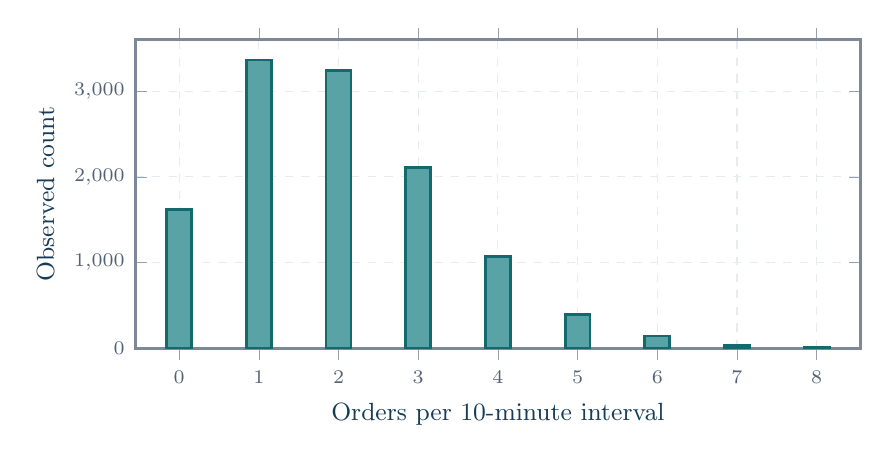
\begin{tikzpicture}
\begin{axis}[
  relayaxis,
  width=.89\linewidth,
  height=5.5cm,
  ybar,
  bar width=9pt,
  ymin=0,
  ymax=3600,
  xlabel={Orders per 10-minute interval},
  ylabel={Observed count},
  xmin=-.55,
  xmax=8.55,
  xtick={0,1,2,3,4,5,6,7,8}
]

\addplot[
  fill=Teal!72,
  draw=DarkTeal
]
coordinates {
  (0,1623)
  (1,3363)
  (2,3240)
  (3,2113)
  (4,1075)
  (5,393)
  (6,144)
  (7,35)
  (8,12)
};

\end{axis}
\end{tikzpicture}

\caption{
Generated normal-operation arrival
frequencies.
The two remaining observations had
nine arrivals each.
The generator is synthetic and
not calibrated to Cathay traffic.
}
\label{fig:arrival}
\end{figure}

\subsection{Monte Carlo convergence}

One earlier independent benchmark,
seed 2026, measured the normal-operation
RELAY v11 cost-reduction estimator
as the paired sample size increased.

\begin{figure}[!htbp]
\centering

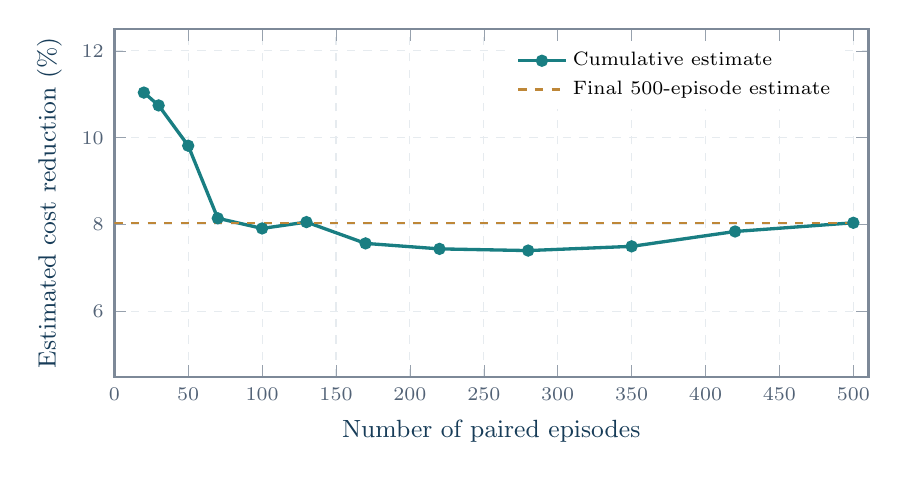
\begin{tikzpicture}
\begin{axis}[
  relayaxis,
  width=.92\linewidth,
  height=6.0cm,
  xmin=0,
  xmax=510,
  ymin=4.5,
  ymax=12.5,
  xlabel={Number of paired episodes},
  ylabel={Estimated cost reduction (\%)},
  legend pos=north east
]

\addplot[
  color=Teal,
  very thick,
  mark=*,
  mark size=1.6pt
]
coordinates {
  (20,11.039)
  (30,10.744)
  (50,9.817)
  (70,8.149)
  (100,7.915)
  (130,8.061)
  (170,7.571)
  (220,7.445)
  (280,7.406)
  (350,7.503)
  (420,7.845)
  (500,8.045)
};

\addplot[
  color=Gold,
  dashed,
  thick,
  domain=0:500
]
{8.045};

\legend{
  Cumulative estimate,
  Final 500-episode estimate
}

\end{axis}
\end{tikzpicture}

\caption{
Sampling convergence in the separate
v11 seed-2026 experiment.
The converged estimate is about 8.05\%.
This is not solver convergence.
}
\label{fig:convergence}
\end{figure}

The reported paired-bootstrap 95\% interval
for that separate experiment was

\[
[7.10\%,8.95\%].
\]

Its result should not be substituted
for the v12 holdout's
8.82\% estimate:
the experiments use different
synthetic random streams.

\subsection{Scenario probabilities and uncertainty}

Let \(s\in\mathcal S\)
index operating regimes
with probabilities \(p_s\).

The scenario-weighted modeled cost is

\begin{equation}
\EE C_\pi
=
\sum_{s\in\mathcal S}
p_s\EE[C_\pi\mid s].
\label{eq:scenario-mix}
\end{equation}

Any such aggregate is meaningful
only after specifying \(p_s\).

The research prototype's illustrative
scenario probabilities were

\[
\begin{array}{c|cccccc}
s&
N&P&C&O&H&D\\
\hline
p_s&
.40&.20&.15&.10&.10&.05
\end{array}
\]

for normal, peak, crew shortage,
cold outage, high capacity
and temporary disruption.

These weights are hypothetical.
They are not empirical Cathay
operating-regime frequencies.

% ============================================================
\section{Recovery Performance and Failure Cases}
% ============================================================

\subsection{Average staging improvement}

The v11 full-cohort experiment
used seed 2026 and measured
mean staging lead-time reductions
relative to FCFS.

\begin{table}[!htbp]
\centering
\caption{
Separate v11 full-cohort
lead-time experiment.
}
\small
\begin{tabular}{@{}lr@{}}
\toprule
Scenario & Mean lead-time reduction \\
\midrule
Normal & 3.53\% \\
Peak & 7.29\% \\
Crew shortage & 0.00\% \\
Cold outage & 1.68\% \\
High capacity & 6.59\% \\
Temporary disruption & 3.70\% \\
\bottomrule
\end{tabular}
\end{table}

These are reductions in
\emph{ground staging lead time},
not a measured speed-up of
flight recovery or actual cargo delivery.

\subsection{A negative recovery result}

A particularly important
counterexample concerns
temporary disruption recovery.

In the separate v11 experiment,
the time required to clear
90\% of the restoration-time backlog
was approximately

\[
22.234\text{ ticks}
\quad\text{for FCFS},
\]

versus

\[
25.596\text{ ticks}
\quad\text{for RELAY v11}.
\]

Hence the relative increase was

\begin{equation}
100
\left(
\frac{25.596}{22.234}-1
\right)
=
\boxed{15.1\%}.
\end{equation}

Although modeled total cost was lower,
this particular recovery-clearance measure
was worse.

\begin{figure}[!htbp]
\centering

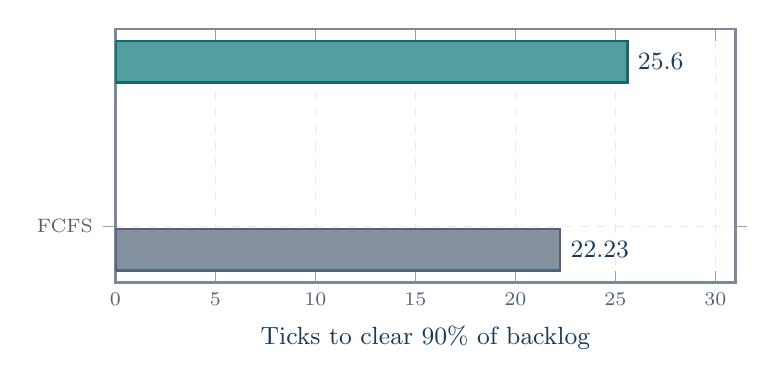
\begin{tikzpicture}
\begin{axis}[
  relayaxis,
  width=.78\linewidth,
  height=4.8cm,
  xbar,
  xmin=0,
  xmax=31,
  xlabel={Ticks to clear 90\% of backlog},
  symbolic y coords={FCFS,RELAY},
  ytick=data,
  enlarge y limits=.4,
  bar width=15pt,
  nodes near coords,
  nodes near coords style={
    font=\small,
    color=Navy
  }
]

\addplot[
  fill=Slate!70,
  draw=Slate
]
coordinates {(22.234,FCFS)};

\addplot[
  fill=Teal!75,
  draw=DarkTeal
]
coordinates {(25.596,RELAY)};

\end{axis}
\end{tikzpicture}

\caption{
A documented negative result:
the v11 policy cleared
90\% of restoration backlog more slowly,
despite improved aggregate modeled cost.
}
\label{fig:recovery-negative}
\end{figure}

This result illustrates why
\emph{recovery quality} must be
defined with multiple metrics.

Relevant metrics include

\[
\begin{aligned}
&\text{decision latency},\\
&\text{time to first feasible recovery},\\
&\text{backlog clearance time},\\
&\text{service completion rate},\\
&\text{unresolved shipment count},\\
&\text{rehandling cost},\\
&\text{tail service loss}.
\end{aligned}
\]

A policy should not be declared
universally superior from
a single aggregate percentage.

% ============================================================
\section{Computational Performance and Software QA}
% ============================================================

\subsection{Finite-column MILP performance}

A separate network-solver test
evaluated 36 bounded synthetic
Model III instances.

The candidate column count
ranged from approximately
9 to 78.

All 36 instances returned the
solver's optimal status
for their modeled finite-column problems.

Reported solver timing was

\[
\operatorname{Median}=5.31\text{ ms},
\]

\[
P_{95}=6.20\text{ ms}.
\]

These times exclude
large portions of end-to-end
data ingestion,
external confirmation,
ground execution and UI latency.

\subsection{Simulation speed and interpretation}

The visual simulation and mathematical
solver use different computational workloads.

In an earlier full-system timing test,
a requested 100-times playback speed
did not yield 100-times
completed mathematical simulation work.

By contrast, the final v12
lightweight five-policy staging engine
recorded approximately

\[
52.42\text{ ticks/s}
\]

over a short local test,
against a nominal requested target
of 50 ticks/s.

The measurement covered only
the simplified five-way staging engine,
not all Models I--III at every tick,
and was not independently
validated on the user's Windows hardware.

\subsection{Correctness checks}

The final v12 selected regression run
reported

\[
\boxed{77/77\text{ passed}}.
\]

The selected tests covered
mathematical components,
data and API contracts,
capacity guards,
five-policy selection,
simulation synchronization
and regression behavior.

Additional reported validation included:

\begin{itemize}[leftmargin=18pt,itemsep=2pt]
\item
500 randomized hybrid-selection constraint cases;
\item
25 legacy benchmark parity fixtures;
\item
native Chromium WebGL2 rendering
for two-, three- and five-world layouts;
\item
shared-input policy advancement and
minimum-two-world selection constraints;
\item
fresh ZIP extraction and selected
functional re-execution;
\item
structural historical-data audit.
\end{itemize}

\researchnote{What 77/77 means.}{
It means that 77 selected automated
tests passed under the tested environment.
It is not a proof of complete correctness,
a full historical test-suite pass,
an airline production certification,
or evidence that all theorem assumptions
have been physically validated.
}

\subsection{Numerical validation levels}

\begin{table}[!htbp]
\centering
\caption{What was validated and at what scope.}
\label{tab:qa}
\small
\begin{tabularx}{\linewidth}{@{}p{34mm}L@{}}
\toprule
Component & Validation scope \\
\midrule
CVaR calculations &
Randomized numerical consistency
within finite synthetic distributions. \\
Model I &
Budget and non-worsening objective
within bounded 2D candidate libraries. \\
Model II &
Finite one-step Bayesian posterior
and information-value identities. \\
Model III &
Finite-column MILP optimality;
small exhaustive comparison fixtures. \\
Shared state &
Event, shipment and clock consistency
in selected API integration scenarios. \\
Five-way comparison &
Common inputs, per-policy state,
capacity checks and policy selection. \\
3D rendering &
Interactive visualization and WebGL2
browser behavior; not certified physics. \\
\bottomrule
\end{tabularx}
\end{table}

% ============================================================
\section{Economics: From Synthetic Gains to ROI}
% ============================================================

\subsection{What the current percentages mean}

A cost improvement such as 11.47\%
means

\[
\frac{
\text{modeled FCFS penalty}
-
\text{modeled Model A penalty}
}{
\text{modeled FCFS penalty}
}
\times100\%.
\]

It does not mean
Cathay's accounting expenses
fell by 11.47\%.

The synthetic ledger contains
unvalidated cost weights.

True savings depend on actual
labor costs, service contracts,
missed connections,
spoilage, rehandling,
customer penalties
and the cost of deploying RELAY.

\subsection{Break-even analysis}

Let

\begin{itemize}[leftmargin=18pt,itemsep=2pt]
\item \(N\) be comparable operating batches per month;
\item \(\Delta C\) be modeled cost units
saved per batch;
\item \(k\) be the independently calibrated
HKD per modeled cost unit;
\item \(F\) be monthly incremental deployment
and operating cost in HKD.
\end{itemize}

Then a hypothetical monthly ROI is

\begin{equation}
ROI=
100
\left(
\frac{N\Delta Ck-F}{F}
\right).
\label{eq:roi}
\end{equation}

Break-even requires

\begin{equation}
k_{\mathrm{BE}}
=
\frac{F}{N\Delta C}.
\label{eq:breakeven}
\end{equation}

\subsection{Illustrative sensitivity example}

Take

\[
N=60,
\qquad
F=\mathrm{HKD}\,20{,}000,
\]

and an illustrative
modeled normal-operation reduction

\[
\Delta C=143.13
\]

synthetic cost units per comparable batch
from the earlier v11 analysis.

Then

\begin{equation}
k_{\mathrm{BE}}
=
\frac{20{,}000}{60(143.13)}
\approx
\mathrm{HKD}\,2.33
\end{equation}

per synthetic unit.

\begin{figure}[!htbp]
\centering

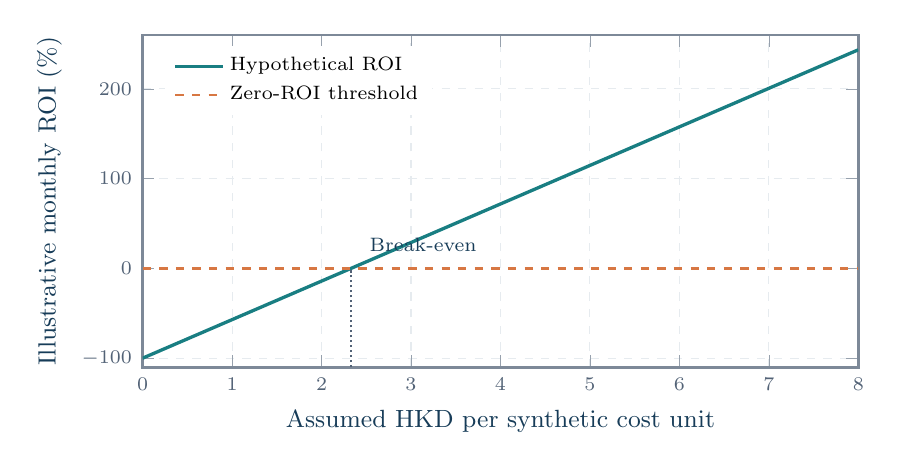
\begin{tikzpicture}
\begin{axis}[
  relayaxis,
  width=.88\linewidth,
  height=5.8cm,
  xmin=0,
  xmax=8,
  ymin=-110,
  ymax=260,
  xlabel={
    Assumed HKD per synthetic cost unit
  },
  ylabel={Illustrative monthly ROI (\%)},
  legend pos=north west
]

\addplot[
  color=Teal,
  very thick,
  domain=0:8,
  samples=80
]
{100*(60*143.13*x/20000-1)};

\addplot[
  color=Orange,
  thick,
  dashed,
  domain=0:8
]
{0};

\addplot[
  color=Slate,
  densely dotted,
  thick
]
coordinates {
  (2.3287,-110)
  (2.3287,0)
};

\node[
  font=\scriptsize,
  anchor=south west,
  color=Navy
]
at (axis cs:2.42,7)
{Break-even};

\legend{
  Hypothetical ROI,
  Zero-ROI threshold
}

\end{axis}
\end{tikzpicture}

\caption{
Illustrative ROI sensitivity.
The chart uses hypothetical
operating volume, deployment cost
and monetary calibration.
It is not a forecast of Cathay savings.
}
\label{fig:roi}
\end{figure}

The real value of \(k\),
actual operating frequency \(N\)
and true deployment cost \(F\)
have not been established.

Accordingly,

\begin{center}
\textbf{\color{Navy}
Real-world monetary ROI remains unknown.
}
\end{center}

\subsection{Where business value may emerge}

A validated future implementation
could create economic value through

\begin{enumerate}[
  label=(\roman*),
  leftmargin=18pt,
  itemsep=2pt
]
\item
fewer avoidable missed service commitments;
\item
reduced rehandling and handling conflict;
\item
better allocation of scarce flight capacity;
\item
fewer unnecessary inspections or switches;
\item
faster identification of safe recovery options;
\item
reduced manual coordination effort;
\item
earlier and more accurate
customer recovery communication.
\end{enumerate}

The first five are direct research hypotheses
linked to the mathematical models.
The last two are product and workflow hypotheses
requiring separate field measurement.

% ============================================================
\section{Production Architecture and Integration}
% ============================================================

\subsection{Current working system}

The final software is a
Python-based local full-stack
research application.

Its principal components are

\begin{itemize}[leftmargin=18pt,itemsep=2pt]
\item FastAPI and typed API contracts;
\item event and versioned state handling;
\item bounded mathematical solvers;
\item five-way synthetic staging policy engine;
\item WebGL2 operational visualizations;
\item Ground, Control Tower and Customer projections;
\item test suites and reproducible benchmark reports.
\end{itemize}

This constitutes a working,
auditable synthetic prototype.

It is not yet a
multi-tenant airline production deployment.

\subsection{Target operational data plane}

A production data plane should distinguish

\begin{table}[!htbp]
\centering
\caption{Data ownership and operational authority.}
\small
\begin{tabularx}{\linewidth}{@{}p{34mm}L@{}}
\toprule
Source & Authorized responsibility \\
\midrule
OAG or equivalent &
External schedules,
connections and flight observations. \\
Carrier inventory &
Bookable space,
allotments and capacity confirmations. \\
Terminal systems &
Physical ULD state,
handling equipment and task completion. \\
Cargo records &
Shipment identity, piece dimensions,
special-cargo requirements and milestones. \\
Safety authority &
Physical load certification,
DG and aircraft/ULD restrictions. \\
RELAY engine &
Decision support, uncertainty,
optimization, explanation and proposal status. \\
\bottomrule
\end{tabularx}
\end{table}

The boundaries are essential:
external schedules cannot silently
overwrite carrier-internal inventory.

\subsection{Target decision transaction}

A robust operational decision should
have a versioned lifecycle

\[
\begin{aligned}
&\text{Proposed}\\
&\quad\downarrow\\
&\text{Internally reviewed}\\
&\quad\downarrow\\
&\text{Externally confirmed}\\
&\quad\downarrow\\
&\text{Operationally executed}\\
&\quad\downarrow\\
&\text{Acknowledged and reconciled}.
\end{aligned}
\]

Each transition requires
a justified authority and
fresh evidence.

Stale recommendations should be
revalidated or rejected.

\subsection{Production control requirements}

Before real use, the system needs

\begin{enumerate}[
  label=\textbf{G\arabic*.},
  leftmargin=20pt,
  itemsep=3pt
]
\item
Authorized, calibrated operational data.
\item
Complete role-based authentication
and customer data isolation.
\item
Carrier-confirmed capacity
and booking status.
\item
Certified ULD and physical
ground-handling feasibility.
\item
Operationally safe action permissions
and human responsibility assignment.
\item
Idempotent external commands,
retries and acknowledged outcomes.
\item
Tamper-evident audit trails,
monitoring and incident recovery.
\item
Shadow-mode validation before
any approved automatic execution.
\end{enumerate}

Passing an internal solver
constraint check is insufficient
to discharge these requirements.

% ============================================================
\section{What Is Complete and What Is Not}
% ============================================================

\begin{table}[!htbp]
\centering
\caption{
Final research-to-production traceability.
}
\label{tab:gaps}
\small
\begin{tabularx}{\linewidth}{@{}p{33mm}p{28mm}L@{}}
\toprule
Requirement &
Current status &
Remaining work \\
\midrule
Three original mathematical formulations &
Research complete &
Empirical assumptions and
deployment prerequisites. \\
Model I bounded risk optimization &
Implemented &
Full certified 3D geometry,
handling paths and stochastic recourse. \\
Model II one-step verification &
Implemented &
Calibrated multi-stage
belief-state control. \\
Model III finite MILP &
Implemented &
Complete candidate generation,
physical certificates and full coupling. \\
Graver/cluster exchange &
Mathematical fixture &
Operational integrated augmentation,
runtime and quality comparisons. \\
Synthetic historical data &
Generated/audited &
Actual source calibration
and representativeness testing. \\
Five staging strategies &
Implemented/tested &
Independent real-world policy validation. \\
Five selectable 3D worlds &
Implemented &
Operationally faithful physical telemetry. \\
Three-perspective UI &
Implemented &
Authenticated real customer
and staff workflows. \\
Economic model &
Sensitivity analysis &
Calibrated HKD costs
and observed pilot outcomes. \\
Production controls &
Not complete &
Security, authorization,
certification and monitored deployment. \\
\bottomrule
\end{tabularx}
\end{table}

\subsection{Why development can stop at v12}

There is a rational distinction between
stopping a hackathon feature cycle
and claiming production completeness.

Version 12 is sufficient to demonstrate:

\begin{itemize}[leftmargin=18pt,itemsep=2pt]
\item
a rigorous research rationale;
\item
nontrivial mathematical optimization;
\item
operational decision alternatives;
\item
reproducible five-policy experiments;
\item
quantified synthetic improvements;
\item
visible adverse cases;
\item
traceable data and model limitations;
\item
an implementable path toward real validation.
\end{itemize}

Further feature expansion using
the same synthetic assumptions
would offer diminishing evidence
of real-world value.

The next major improvement should be
\emph{external validity},
not another digital-twin animation.

% ============================================================
\section{A Falsifiable Real-World Validation Plan}
% ============================================================

\subsection{Choose a narrow use case}

A first pilot should focus on
one concrete, measurable recovery class,
for example:

\begin{quote}
\small
A disrupted outbound shipment at HKG
with a confirmed service deadline,
a small set of feasible alternative flights,
limited verified ground resources,
and an explicit physical/booking approval chain.
\end{quote}

This is more defensible than
claiming general optimization of
all cargo operations at once.

\subsection{Shadow-mode evaluation}

RELAY should initially recommend
without executing.

For each real decision epoch, record:

\begin{itemize}[leftmargin=18pt,itemsep=2pt]
\item the information actually available;
\item the human baseline recommendation;
\item RELAY's recommended action;
\item all alternative options considered;
\item solver feasibility, bound and runtime;
\item subsequent actual event outcomes;
\item customer, service and financial outcomes.
\end{itemize}

No future observation may leak
into the historical decision snapshot.

\subsection{Primary endpoints}

A pilot could pre-register

\begin{align}
\text{Service gain}
&=
Q_{\mathrm{RELAY}}-Q_{\mathrm{baseline}},
\\
\text{Recovery-time gain}
&=
1-
\frac{
T_{\mathrm{RELAY}}
}{
T_{\mathrm{baseline}}
},
\\
\text{Cost gain}
&=
1-
\frac{
C_{\mathrm{RELAY}}
}{
C_{\mathrm{baseline}}
}.
\end{align}

These should be reported with
appropriate confidence intervals,
sample sizes and clear denominators.

Also report

\[
\PP(
C_{\mathrm{RELAY}}>
C_{\mathrm{baseline}}
)
\]

and tail-risk measures.

\subsection{Required ablations}

To identify the source of benefit,
compare at least

\begin{enumerate}[
  label=(\Alph*),
  leftmargin=20pt,
  itemsep=2pt
]
\item FCFS or current operational baseline;
\item Model III global allocation alone;
\item Model III with Model I physical filtering;
\item Model III with Model II
expiry-aware verification;
\item full coordinated decision support;
\item candidate cluster/Graver augmentation
against exact MILP, under equal budgets.
\end{enumerate}

Ablations are necessary because
success of the five-way staging benchmark
does not establish the incremental value
of all three research models.

\subsection{Hypotheses and failure thresholds}

The eventual research paper should test
hypotheses such as:

\begin{itemize}[leftmargin=18pt,itemsep=2pt]
\item
risk-aware physical arrangements reduce
verified recourse cost
without violating a nominal-efficiency budget;
\item
expiry-aware verification reduces
avoidable switches
relative to fixed inspection rules;
\item
global capacity allocation improves
service-weighted recovery
relative to independent rerouting;
\item
coordinated decisions reduce
actual missed-service and handling cost;
\item
recommendation latency stays below
the operationally useful decision window.
\end{itemize}

Failure to establish these effects
under real data should be reported
as a negative or inconclusive result,
not concealed by synthetic averages.

% ============================================================
\section{Threats to Validity}
% ============================================================

\subsection{Synthetic-data dependence}

The measured gains depend on
Poisson arrivals,
task templates,
service penalties,
duration distributions,
capacity settings
and disruption rules.

These assumptions may not represent
actual cargo terminal operations.

\subsection{Objective mismatch}

A synthetic penalty objective
can select a policy that is
cheaper according to the model
but inferior under actual
contractual service priorities.

The demonstrated cost/SLA frontier
makes this limitation visible.

\subsection{Incomplete physical semantics}

The three-dimensional display
is a state-driven procedural
representation.

It is not a verified digital replica
of Cathay Cargo Terminal,
and it does not establish
collision-free aircraft or equipment
movement.

\subsection{Incomplete mathematical coupling}

The final runtime does not
fully resolve all possible
belief, packing, capacity and
execution feedback loops.

In particular, contingent
verification decisions require
additional shared-network reoptimization
to realize the full original theory.

\subsection{Limited computational scale}

MILP optimality results refer
to bounded candidate sets.

Small solver times do not imply
similar performance for
large airline networks.

Similarly, 100-times
lightweight staging playback
does not imply 100-times
full stochastic optimization.

\subsection{Real-world safety}

Unknown permissions,
physical loading restrictions
and booking availability
cannot be made feasible
by changing an objective penalty.

Mandatory safety restrictions
remain hard constraints
independent of business value
\cite{iatauld}.

% ============================================================
\section{Research Contributions and Interpretation}
% ============================================================

The completed project makes
three types of contribution.

\subsection{Mathematical contribution}

The three underlying research papers
provide:

\begin{enumerate}[
  label=(\roman*),
  leftmargin=18pt,
  itemsep=3pt
]
\item
budgeted recovery-risk dominance
and a quantitative criterion
for strict improvement;
\item
an exact decomposition of
verification value into
information, option change,
delay and inspection cost;
\item
a certified algebraic representation
of feasible global recovery exchanges,
with Graver-based augmentation guarantees.
\end{enumerate}

These are mathematical statements
under their explicit assumptions.

They do not depend on a
3D visualization being present.

\subsection{Engineering contribution}

RELAY combines

\begin{itemize}[leftmargin=18pt,itemsep=2pt]
\item a versioned event model;
\item bounded executable optimization;
\item explicit provisional/confirmed states;
\item a synchronized three-perspective interface;
\item a five-policy common-input staging simulator;
\item reproducible benchmark and QA artifacts.
\end{itemize}

The engineering contribution is
a working research demonstration
of how decision intelligence can be
made inspectable and operationally legible.

\subsection{Experimental contribution}

The final holdout demonstrates
that policy choice matters.

Under normal modeled conditions:

\[
\begin{aligned}
S_{\mathrm{ModelA}}&=11.47\%,\\
Q_{\mathrm{ModelA}}&=64.04\%,\\
S_{\mathrm{EDF}}&=17.53\%,\\
Q_{\mathrm{EDF}}&=56.64\%.
\end{aligned}
\]

These outcomes support
a multiobjective decision-support
interpretation rather than a
single universally optimal heuristic.

Under severe crew shortage,
the newer policies fall back to
FCFS and show no improvement.

Negative cases remain central
to the scientific conclusion.

% ============================================================
\section{Conclusion}
% ============================================================

The fundamental idea behind RELAY
is that an operational recovery decision
should be evaluated not only by its
immediate cost,
but also by the opportunities
it preserves or destroys.

Model I formalizes the value of
physically recoverable arrangements.
Model II formalizes the decision value
of timely verification.
Model III formalizes the need for
globally coordinated allocation
of finite recovery resources.

Together, they define a coherent
research program:

\begin{center}
\textbf{\color{Navy}
Physical feasibility
\(\longrightarrow\)
Information-aware decisions
\(\longrightarrow\)
Global capacity recovery.
}
\end{center}

The software development journey
from v1 to v12 transformed these
formulations into a working
synthetic decision-support prototype
with synchronized operational views,
five comparable scheduling policies
and reproducible experiments.

The final benchmark demonstrates
measurable, scenario-dependent
improvements in modeled
cost, service quality and tail risk.
It also demonstrates meaningful
trade-offs and failure cases.

The crucial conclusion is therefore
neither that the concept has failed
nor that airline-wide production value
has already been proven.

Rather, the project has established
a sufficiently concrete mathematical,
software and experimental basis
to justify a narrowly scoped,
authorized real-data pilot.

\begin{center}

\vspace{5pt}

{\large\bfseries\color{Navy}
Buy the Future Optionality.
}

\vspace{3pt}

{\normalsize
Optimize what can be done now,
without unnecessarily destroying
what may need to be done next.
}

\end{center}

% ============================================================
\appendix
% ============================================================

\section{Detailed Benchmark Data}

\subsection{Full six-scenario cost-reduction matrix}

All values below are percentages relative
to the corresponding FCFS mean.

\begin{table}[!htbp]
\centering
\caption{
Final five-policy, six-scenario
synthetic cost matrix.
}
\small
\begin{adjustbox}{max width=\linewidth}
\begin{tabular}{@{}lrrrrr@{}}
\toprule
Scenario &
FCFS &
v10 &
v11 &
Model A &
EDF \\
\midrule
Normal & 0.0000 & 6.5076 & 8.8165 & 11.4666 & 17.5252\\
Peak & 0.0000 & 0.4034 & 17.2159 & 18.1751 & 22.2399\\
Crew shortage & 0.0000 & -0.3659 & 0.0000 & 0.0000 & 0.0000\\
Cold outage & 0.0000 & 1.1519 & 2.4955 & 2.7936 & 3.7367\\
High capacity & 0.0000 & 11.1919 & 10.6157 & 14.7489 & 23.9535\\
Temporary disruption & 0.0000 & 1.9277 & 10.0726 & 10.8790 & 15.8806\\
\bottomrule
\end{tabular}
\end{adjustbox}
\end{table}

\subsection{Normal-operation relative costs}

The final normal-operation
FCFS average was

\[
\overline C_{\mathrm{FCFS}}
=
1946.8353.
\]

The remaining mean costs were

\begin{align*}
\overline C_{\mathrm{v10}} &=1820.1423,\\
\overline C_{\mathrm{v11}} &=1775.1927,\\
\overline C_{\mathrm{ModelA}} &=1723.6003,\\
\overline C_{\mathrm{EDF}} &=1605.6485.
\end{align*}

Substitution into
\eqref{eq:savings}
reproduces the displayed
normal-operation cost percentages,
subject to rounding.

\subsection{Seed and experiment separation}

\begin{table}[!htbp]
\centering
\caption{
Distinct evaluation datasets
used during development.
}
\small
\begin{tabularx}{\linewidth}{@{}p{25mm}p{23mm}L@{}}
\toprule
Experiment &
Seed &
Purpose \\
\midrule
v10 original &
Earlier pinned runs &
21-tick partial-window
staging comparison. \\
v11 full cohort &
2026 &
Complete cohort;
three-policy evaluation,
CI and recovery metrics. \\
v11 replication &
707 &
Second synthetic seed
under the same generator. \\
v12 final holdout &
9099 &
Five policies,
six scenarios,
500 paired episodes per scenario. \\
\bottomrule
\end{tabularx}
\end{table}

Different experimental regimes
must not be combined into
a single confidence interval
without a valid common estimand.

% ============================================================
\section{Mathematical and Engineering Audit Checklist}
% ============================================================

\begin{longtable}{@{}p{48mm}p{22mm}p{84mm}@{}}
\caption{
Research-to-product validation register.
}
\\
\toprule
Requirement & Status & Required interpretation \\
\midrule
\endfirsthead

\toprule
Requirement & Status & Required interpretation \\
\midrule
\endhead

Model I CVaR formula &
Tested &
Finite synthetic loss vectors only. \\

Model I nominal budget &
Tested &
Candidate-library budget,
not a full physical arrangement certificate. \\

3D ULD contour &
Incomplete &
Requires aircraft/ULD-specific
certified geometry. \\

Safe physical rehandling &
Incomplete &
Needs motion paths,
restraint and resource feasibility. \\

Model II Bayes identity &
Tested &
Finite one-step synthetic loss models. \\

Model II sequential controller &
Incomplete &
Requires calibrated transition kernels
and operational decisions over time. \\

Model III finite MILP &
Tested &
Optimality relative to modeled
candidate columns and constraints. \\

Cluster exchange certificate &
Research &
Mathematical construction;
not deployed as full operational search. \\

Cross-model coupling &
Partial &
Shared state and safety gates exist;
not all contingency branches are jointly re-solved. \\

Historical data integrity &
Tested &
Synthetic schema and reference checks passed. \\

Historical statistical realism &
Unvalidated &
Requires actual airline observations. \\

OAG live integration &
Not enabled &
Synthetic adapter only;
licensed access required. \\

Five-way staging comparison &
Tested &
Identical synthetic input streams
and separate policy states. \\

Customer state projection &
Partial &
Works with synthetic evidence;
no live airline confirmation. \\

Local API security &
Limited &
Not sufficient for public
or multi-tenant deployment. \\

Real-world economic ROI &
Unknown &
Requires calibrated costs and pilot data. \\

\bottomrule

\end{longtable}

% ============================================================
\section{Reproducibility Notes}
% ============================================================

The final software release contains
reproducible reports and source code,
including:

\begin{itemize}[leftmargin=18pt,itemsep=2pt]
\item
final five-policy holdout summary;
\item
episode-level five-policy results;
\item
three-model source implementations;
\item
synthetic historical flight and cargo records;
\item
QA tests and engineering reports;
\item
versioned digital-twin interfaces.
\end{itemize}

The final benchmark can be reproduced
from the version-12 application
using its built-in benchmark module.

A representative project command is

\begin{verbatim}
python -m v12.benchmark \
  --episodes 500 \
  --seed 9099 \
  --output reports/reproduction
\end{verbatim}

This command requires the original
RELAY v12 source tree and its
installed dependencies.
The present LaTeX document itself
has no external data or image dependencies.

For faithful replication, preserve:

\begin{itemize}[leftmargin=18pt,itemsep=2pt]
\item exact software revision;
\item input generator configuration;
\item random seed;
\item policy implementations;
\item resource and eligibility constraints;
\item accounting horizon;
\item cost and service definitions;
\item original episode-level output.
\end{itemize}

% ============================================================
\begin{thebibliography}{99}
% ============================================================

\bibitem{relaymodel1}
RELAY Research Team.
\newblock
\emph{Recovery-Aware Cargo Arrangement:
An Improvement Theorem, a Two-Stage Model,
and a Computed Example}.
\newblock
Model I mathematical research draft,
22 October 2026.

\bibitem{relaymodel2}
RELAY Research Team.
\newblock
\emph{PIVOT:
The Decision Value of Verification Before Recovery}.
\newblock
Model II mathematical research proposal,
22 October 2026.

\bibitem{relaymodel3}
RELAY Research Team.
\newblock
\emph{RELAY Model III:
Certified Cluster Exchanges---From Local Cargo Recovery
to Global Integer and Stochastic Optimisation}.
\newblock
Mathematical research proposal,
22 October 2026.

\bibitem{rockafellar2000}
R.~T. Rockafellar and S. Uryasev.
\newblock
Optimization of Conditional Value-at-Risk.
\newblock
\emph{Journal of Risk},
2(3):21--41, 2000.
\newblock
\url{https://doi.org/10.21314/JOR.2000.038}.

\bibitem{rockafellar2002}
R.~T. Rockafellar and S. Uryasev.
\newblock
Conditional Value-at-Risk for General Loss Distributions.
\newblock
\emph{Journal of Banking \& Finance},
26:1443--1471, 2002.

\bibitem{blackwell}
D. Blackwell.
\newblock
Equivalent Comparisons of Experiments.
\newblock
\emph{Annals of Mathematical Statistics},
24(2):265--272, 1953.

\bibitem{smallwood}
R.~D. Smallwood and E.~J. Sondik.
\newblock
The Optimal Control of Partially Observable
Markov Processes over a Finite Horizon.
\newblock
\emph{Operations Research},
21(5):1071--1088, 1973.

\bibitem{fomin2002}
S. Fomin and A. Zelevinsky.
\newblock
Cluster Algebras I: Foundations.
\newblock
\emph{Journal of the American Mathematical Society},
15:497--529, 2002.

\bibitem{fomin2007}
S. Fomin and A. Zelevinsky.
\newblock
Cluster Algebras IV: Coefficients.
\newblock
\emph{Compositio Mathematica},
143:112--164, 2007.

\bibitem{deloera}
J.~A. De Loera, R. Hemmecke and M. K\"oppe.
\newblock
\emph{Algebraic and Geometric Ideas
in the Theory of Discrete Optimization}.
\newblock
SIAM, 2013.

\bibitem{hooker}
J.~N. Hooker.
\newblock
Planning and Scheduling by
Logic-Based Benders Decomposition.
\newblock
\emph{Operations Research},
55(3):588--602, 2007.

\bibitem{onerecord}
International Air Transport Association.
\newblock
\emph{ONE Record Standard:
Data Model, API and Security Specifications}.
\newblock
\url{https://www.iata.org/one-record}.
\newblock
Specifications available at
\url{https://iata-cargo.github.io/ONE-Record/}.

\bibitem{oagportal}
OAG.
\newblock
\emph{Flight Info API and Developer Portal}.
\newblock
\url{https://developers.oag.com/}.
\newblock
Public product overview:
\url{https://www.oag.com/flight-info-api}.

\bibitem{iatauld}
International Air Transport Association.
\newblock
\emph{Unit Load Devices:
Operational Safety and Airworthiness}.
\newblock
\url{https://www.iata.org/uld}.

\bibitem{relayv12}
RELAY Research and Engineering Team.
\newblock
\emph{RELAY Fusion v12:
Final Technical Audit, Benchmark Results and Handoff}.
\newblock
Internal reproducible synthetic research artifacts,
11 November 2026.

\end{thebibliography}

\vspace{5pt}

\begin{center}
{\color{RuleGray}\rule{0.70\linewidth}{0.5pt}}

{\small\itshape
RELAY --- Buying Future Optionality
}

{\footnotesize
Mathematical research
\(\cdot\)
Synthetic evidence
\(\cdot\)
Operational validation pathway
}

\end{center}

\end{document}
